% tATOguide.tex
% v1.2 released April 2014

\documentclass[letterpaper]{tATO2e}

\usepackage{subfigure}% Support for small, `sub' figures and tables
%\usepackage[nolists,nomarkers]{endfloat}
%\usepackage[longnamesfirst,sort]{natbib}% Citation support using natbib.sty
%\bibpunct[, ]{(}{)}{;}{a}{,}{,}% Citation support using natbib.sty

\usepackage[natbibapa]{apacite}% Citation support using apacite.sty. Commands using natbib.sty MUST be deactivated first!
\usepackage{color}
\usepackage{nohyperref}
\usepackage{url}

\begin{document}

%\jvol{00} \jnum{00} \jyear{2014} \jmonth{April}

%\articletype{GUIDE}% NOT REQUIRED IN A RESEARCH ARTICLE

\title{Storm surges in the Strait of Georgia simulated with a regional model}

\author{Nancy Soontiens$^{1}$$^{\ast}$\thanks{$^\ast$Corresponding author's email: nsoontie@eos.ubc.ca
\vspace{6pt}}, Susan E. Allen$^{1}$,  Doug Latornell$^{1}$,  Kate Le Sou\"{e}f$^{1}$, Idalia Machuca$^{1}$,\\ Jean-Philippe Paquin$^{2}$,
Youyu Lu$^{3}$, Keith Thompson$^{2}$, Vasily Korabel$^{2}$
\\\vspace{6pt}  $^{1}${\em{University of British Columbia}};
$^{2}${\em{Dalhousie University}};
$^{3}${\em{Bedford Institute of Oceanography}}\\\received{v1.2 released April 2014} }

\maketitle

\begin{abstract}
The Strait of Georgia is a large, semi-enclosed body of water between Vancouver Island and the mainland of British Columbia connected to the Pacific Ocean via the Strait of Juan de Fuca at the south and Johnstone Strait at the north. During the winter months, coastal communities in the Strait of Georgia are at risk to flooding caused by storm surges, a natural hazard that can occur when a strong storm coincides with high tide. This investigation produces storm surge hindcasts using a three-dimensional numerical ocean model for the Strait of Georgia and the surrounding bodies of water (Strait of Juan de Fuca, Puget Sound, and Johnstone Strait) collectively known as the Salish Sea. The numerical model employs the Nucleus for European Modelling of the Ocean (NEMO) architecture in a regional configuration. The model is evaluated through comparisons of tidal elevation harmonics and storm surge water levels with observations. Important forcing factors contributing to storm surges have been assessed. It is shown that the surge entering the domain from the Pacific Ocean contributes most significantly to the variability. Comparisons between simulations with high resolution and low resolution atmospheric forcing further emphasize this point. In addition, local wind patterns cause a slight increase in surge amplitude on the mainland side of the Strait of Georgia when compared to the Vancouver Island coastal areas during a major wind storm on Dec 15, 2006. Generally, surge amplitudes are found to be greater within the Strait of Georgia when compared to amplitudes in the Strait of Juan de Fuca.
\end{abstract}

\begin{keywords}storm surge; Strait of Georgia; Salish Sea; numerical modelling; spatial variation
\end{keywords}

\section{Introduction}\label{sec:intro}


%some general intro paragraph here. Need something about SoG size, geography, islands, sills, rivers, tides....
The Strait of Georgia is a strongly stratified, semi-enclosed body of water located between Vancouver Island and the mainland of British Columbia. It is part of a larger system of waterways collectively known as the Salish Sea and is connected to the Pacific Ocean via the Strait of Juan de Fuca and Johnstone Strait (Figure \ref{fig:domain}). At its southern end, the Strait of Georgia is connected to the Strait of Juan de Fuca through several passages, the largest being Haro Strait. The San Juan and Gulf Islands are scattered throughout these passages where complex bathymetry and steep topographic slopes induce vigorous tidal mixing.  Mixed diurnal and semi-diurnal tides are found throughout most of the Salish Sea but a semi-diurnal amphidrome is present nearby Victoria, where the tides are mainly diurnal \citep{thomson1981oceanography}. This system is home to several large coastal communities, such as Vancouver and Victoria, serves as a waterway for commercial traffic and recreational use, and supports a large and active fishing industry.   

%my attempt at physical oceanography in SoG- Susan feel free to edit.
%Several features related to the physical oceanography of this region render it a challenge to model numerically. The outflow from the Fraser River in the late spring is the primary source of fresh water within the Strait of Georgia and leads to large vertical density gradients in the summer months \citep{thomson1981oceanography}. Additionally, strong tidal mixing through the San Juan and Gulf Islands produces horizontal density gradients that separate the saline waters of the Strait of Juan de Fuca and the fresher water of the Strait of Georgia. It is important to accurately represent the vertical mixing in this region as it sets the rate of export of fresh water through estuarine circulation \citep{masson2004modelling}. The strong tidal currents through the narrow channels of the north, such as Discovery Passage and Johnstone Strait, set a fairly restrictive time step and impose a particular challenge for numerical models. Several modelling efforts for this region exist, varying in choices of grid structure, mixing parametrizations, and domain. 

%intro to storm surges
Many coastal communities in the Strait of Georgia are at risk of flooding and property damage caused by storm surges, a natural hazard arising from the combination of a strong wind storm and high tide. The low atmospheric pressure associated with a storm acts as an inverse barometer elevating the sea level. This effect in combination with strong winds pushing water up against the coast can cause flooding, particularly if the storm occurs during an unusually high tide.  There is also a small contribution to increased sea level due to positive sea surface height anomalies propagating northward from the equator along the eastern Pacific coast during El Nino years \citep{strub2002altimeter}. Communities in the Strait of Georgia are particularly susceptible to storm surges in the winter months when there is an increased propensity for storms and a higher mean sea level caused by southeasterly winds and geostrophic adjustment \citep{danard2003storm}. In the summer months, the wind direction changes to northwesterly and mean sea level is lower. In British Columbia waters, the largest tidal ranges occur in June and December at the summer and winter solstices \citep{thomson1981oceanography}. The highest water levels are observed in the winter around the perigean spring tide or ``King" tide, when the sun and moon are aligned with the Earth and the moon is at its perigee. Storm surges in the Strait of Georgia are typically observed between November and February \citep{forseth2006adaptation}. Flooding caused by a storm surge is most likely to occur during a high spring tide \citep{abeys2011extreme}. 

Coastal communities can prepare for and respond to storm surge hazards using predictions from storm surge models to determine if flooding conditions are probable. Like coastal ocean models, some of the complexity of a storm surge model depends on the properties of the geographic location of interest. In shallow regions, it is important to include the effects of wetting and drying which allows grid cells to alternate between land and water depending on the modelled sea surface height and depth \citep{hubbert1999storm, weisberg2006hurricane}.  Other regions require modelling over a very large domain since non-local effects from the open sea may influence surge propagation \citep{mercer2002barotropic, weisberg2006hurricane, lane2009verification}. Such large domains typically use nested or unstructured grids to resolve the details of complicated coastlines. Appropriate treatment of rivers \citep{flather1994storm}, accurate bathymetry and the inclusion surface waves \citep{xu2010storm} have also been identified as important.  Most of these models neglect the effects of stratification by treating the ocean as a constant temperature and salinity. An accurate forecast of the meteorological conditions at the ocean surface is of course essential in the generation of useful storm surge forecasts.

%storm surge modelling
Storm surge modelling in the Strait of Georgia dates back to \citet{crean1988mathematical} who used a barotropic finite difference model. Their work is highlighted in reviews of storm surges in Canadian waters \citep{murty1995storm, danard2003storm}.  Compared to eastern Canada \citep{gray1984preliminary, bernier2006predicting,bobanovic2006forecasting, bernier2007tide, bernier2010tide}, relatively little has been published on storm surge modelling on the west coast of Canada in recent years. However, a storm surge forecasting program is currently operating over a domain that covers the entire British Columbia coastline \citep{StormBC}. Further, a statistical overview of past surge events in British Columbia waters suggests an increase in extreme water level events during warm El Nino periods \citep{abeys2011extreme}.

%overview oF SoG/Salish Sea models
The early modelling work of \citet{crean1988mathematical}, \citet{crean1988numerical} and \citet{stronach1993update} resulted in a series of models covering the Strait of Juan de Fuca, the Strait of Georgia, and Puget Sound using a finite difference discretization of the equations of motion. %A barotropic version of their model was used to reproduce storm surge water level elevations with reasonable accuracy, however, this barotropic version did not include the effects of fresh water entering the system from rivers. Later, a baroclinic version of their model examined residual circulation and fresh water flushing rates \citep{stronach1993update, marinone1996model}.
These models pointed to an important connection between the model's bottom friction parametrization and the location and amplitude of the M$_2$ amphidrome. They found that a local increase in the bottom friction coefficient, typically from 0.002 to 0.004 in the baroclinic model, especially in the vicinity of Haro Strait, was necessary in order to adequately reproduce the observed M$_2$ tidal amplitudes and phase lags in the Strait of Georgia \citep{stronach1993update}. Without local adjustments to the bottom friction their M$_2$ amplitudes were too low and the M$_2$ tidal phases were too large in the Strait of Georgia \citep{crean1988mathematical}. Local adjustments to bottom friction were applied in both their barotropic and baroclinic models.  Other studies over a similar domain, such as the barotropic finite element model of \citet{foreman1995tidal}, have avoided local increases in bottom friction although their domain did not include Puget Sound and the northern Strait of Georgia. \citet{foreman2004m} assimilated tide gauge harmonics to study M$_2$ tidal dissipation without local changes to the bottom friction in a two-dimensional finite element model that did not include baroclinic effects. 

More recently, modelling studies have focused on baroclinic features. \citet{masson2004modelling} used the Princeton Ocean Model (POM) in a regional mode to examine the seasonal variability of deep water properties in the Strait of Georgia and noted a strong sensitivity to vertical mixing over the sills. This model employed a sigma or terrain-following vertical coordinate system leading to spurious diapycnal mixing since, numerically, the lateral mixing is computed on sigma levels which may intersect isopycnals in the presence of steep topography. 
%A finite volume model on an unstructured grid by \citet{yang2010multi} involved a truncated domain with an open boundary in the northern Strait of Georgia, where under predictions in the M$_2$ tidal phase over most of their domain were suggested to be caused by an inaccurate representation of the tides at their northern boundary. 
\citet{sutherland2011model} employed the Regional Ocean Modelling System (ROMS) to study estuarine circulation in the Salish Sea with a model domain that extended outside the Strait of Juan de Fuca into the Pacific Ocean and up to the northern Strait of Georgia. They noted that their semi-diurnal amplitudes were generally too low. An updated version of this model produced high surface temperatures in the Strait of Juan de Fuca, suggesting too little mixing within the Salish Sea \citep{giddings2014hindcasts}. Smaller domains have also been considered; notably, the passageways through the Discovery Islands north of the Strait of Georgia have been modelled baroclinically by \citet{foreman2012circulation} with the Finite Volume Coastal Ocean Model (FVCOM) pointing to difficulties in reproducing baroclinic currents on their grid.  Accurate reproduction of observed tidal amplitudes and phases and appropriate treatment of mixing is a recurring difficulty in modelling this region.

This article presents the development of a three-dimensional numerical ocean model for the Strait of Georgia and its skill in simulating storm surge hindcasts. To complement previous barotropic storm surge modelling in this region, this model employs a higher resolution and includes the effect of stratification and rivers. However, wetting and drying is not represented. Model evaluation has focused on regions where the near-coast slopes are steep and so wetting and drying effects are believed to be unimportant. A detailed overview of the model configuration and domain is provided in section \ref{sec:config}. That section also describes open and surface boundary conditions as well as choices in grid structure and mixing parametrizations. Next, section \ref{sec:model} presents an evaluation of model performance through comparisons of tidal amplitudes and phases with observations. The model's skill in producing storm surge hindcasts is assessed in section \ref{sec:storm}. Several simulations comparing the effects of different forcing conditions are also discussed. Finally, a summary and discussion of future research goals is provided in section \ref{sec:diss}.  

\section{Model Description}\label{sec:config}

We have used the Nucleus for European Modelling of the Ocean (NEMO) framework in its regional configuration \citep{madec2012nemo} to develop an ocean model for the Salish Sea. NEMO is a highly modular tool used for studying ocean physics, ocean-ice interactions, and the bio-geochemical properties of the ocean. NEMO's ocean core solves the three-dimensional hydrostatic equations of motion for an incompressible fluid under the Boussinesq approximation on a structured computational grid. Although not used in the present work, NEMO's options for grid nesting and bio-geochemical coupling make it a useful tool for studying the complex physics and bio-geochemical interactions within the Strait of Georgia. This work focuses on the physical configuration of the Salish Sea model, in particular, determining appropriate forcing and boundary conditions for accurate reproduction of tidal amplitudes and phases as well as storm surge elevations. Future work will include bio-geochemical coupling and data assimilation. NEMO version 3.4 was used in this study.

The modelled domain extends from the Strait of Juan de Fuca to Puget Sound to Johnstone Strait (Figure \ref{fig:domain}). Bathymetry from the Cascadia physiography data set \citep{haugerud1999digital} was smoothed to limit large changes in depth across grid cells, so that $\Delta h/\bar{h} \leq 0.8$, where $\Delta h$ is the difference in depth between two adjacent grid cells and $\bar{h}$ is their average depth. For model stability, additional smoothing at the Strait of Juan de Fuca western boundary was imposed to achieve constant depth across the first ten grid cells. As depicted in Figure \ref{fig:domain}, the numerical grid is rotated $29^{\circ}$ counter-clockwise of North in order to maintain computational efficiency since currents within the Strait of Georgia are mainly aligned with this rotated axis. 

The curvilinear orthogonal numerical grid has been divided into 398 by 898 by 40 grid cells, which results in an almost uniform horizontal resolution with grid spacing approximately 440 m by 500 m. The 40 vertical $z$-levels were stretched gradually in order to achieve higher resolution in the surface layer, with 1 m vertical grid spacing down to about 10 m in depth. Below 10 m the grid was stretched to a maximum grid spacing of 27 m in the lowest layer. At the bottom boundary, partial $z$-levels were used in order to limit large changes in bathymetry across grid cells \citep{madec2012nemo}. 

In addition to the equations of motion, a prognostic equation for the sea surface height is solved at each time step. The inclusion of the sea surface height equation requires a fairly restrictive time step due to the presence of high speed surface gravity waves. As such, the split-explicit time stepping algorithm is employed, where the free surface and barotropic equations are solved with a smaller time step than that used for the other variables. The model baroclinic time step and barotropic time step are 10 s and 2 s respectively. Small vertical grid spacing and large vertical velocities in the Boundary Pass and Haro Strait region impose a fairly restrictive baroclinic time step through the vertical Courant-Friedrichs-Lewy (CFL) condition.


\begin{figure}[h]
\centering
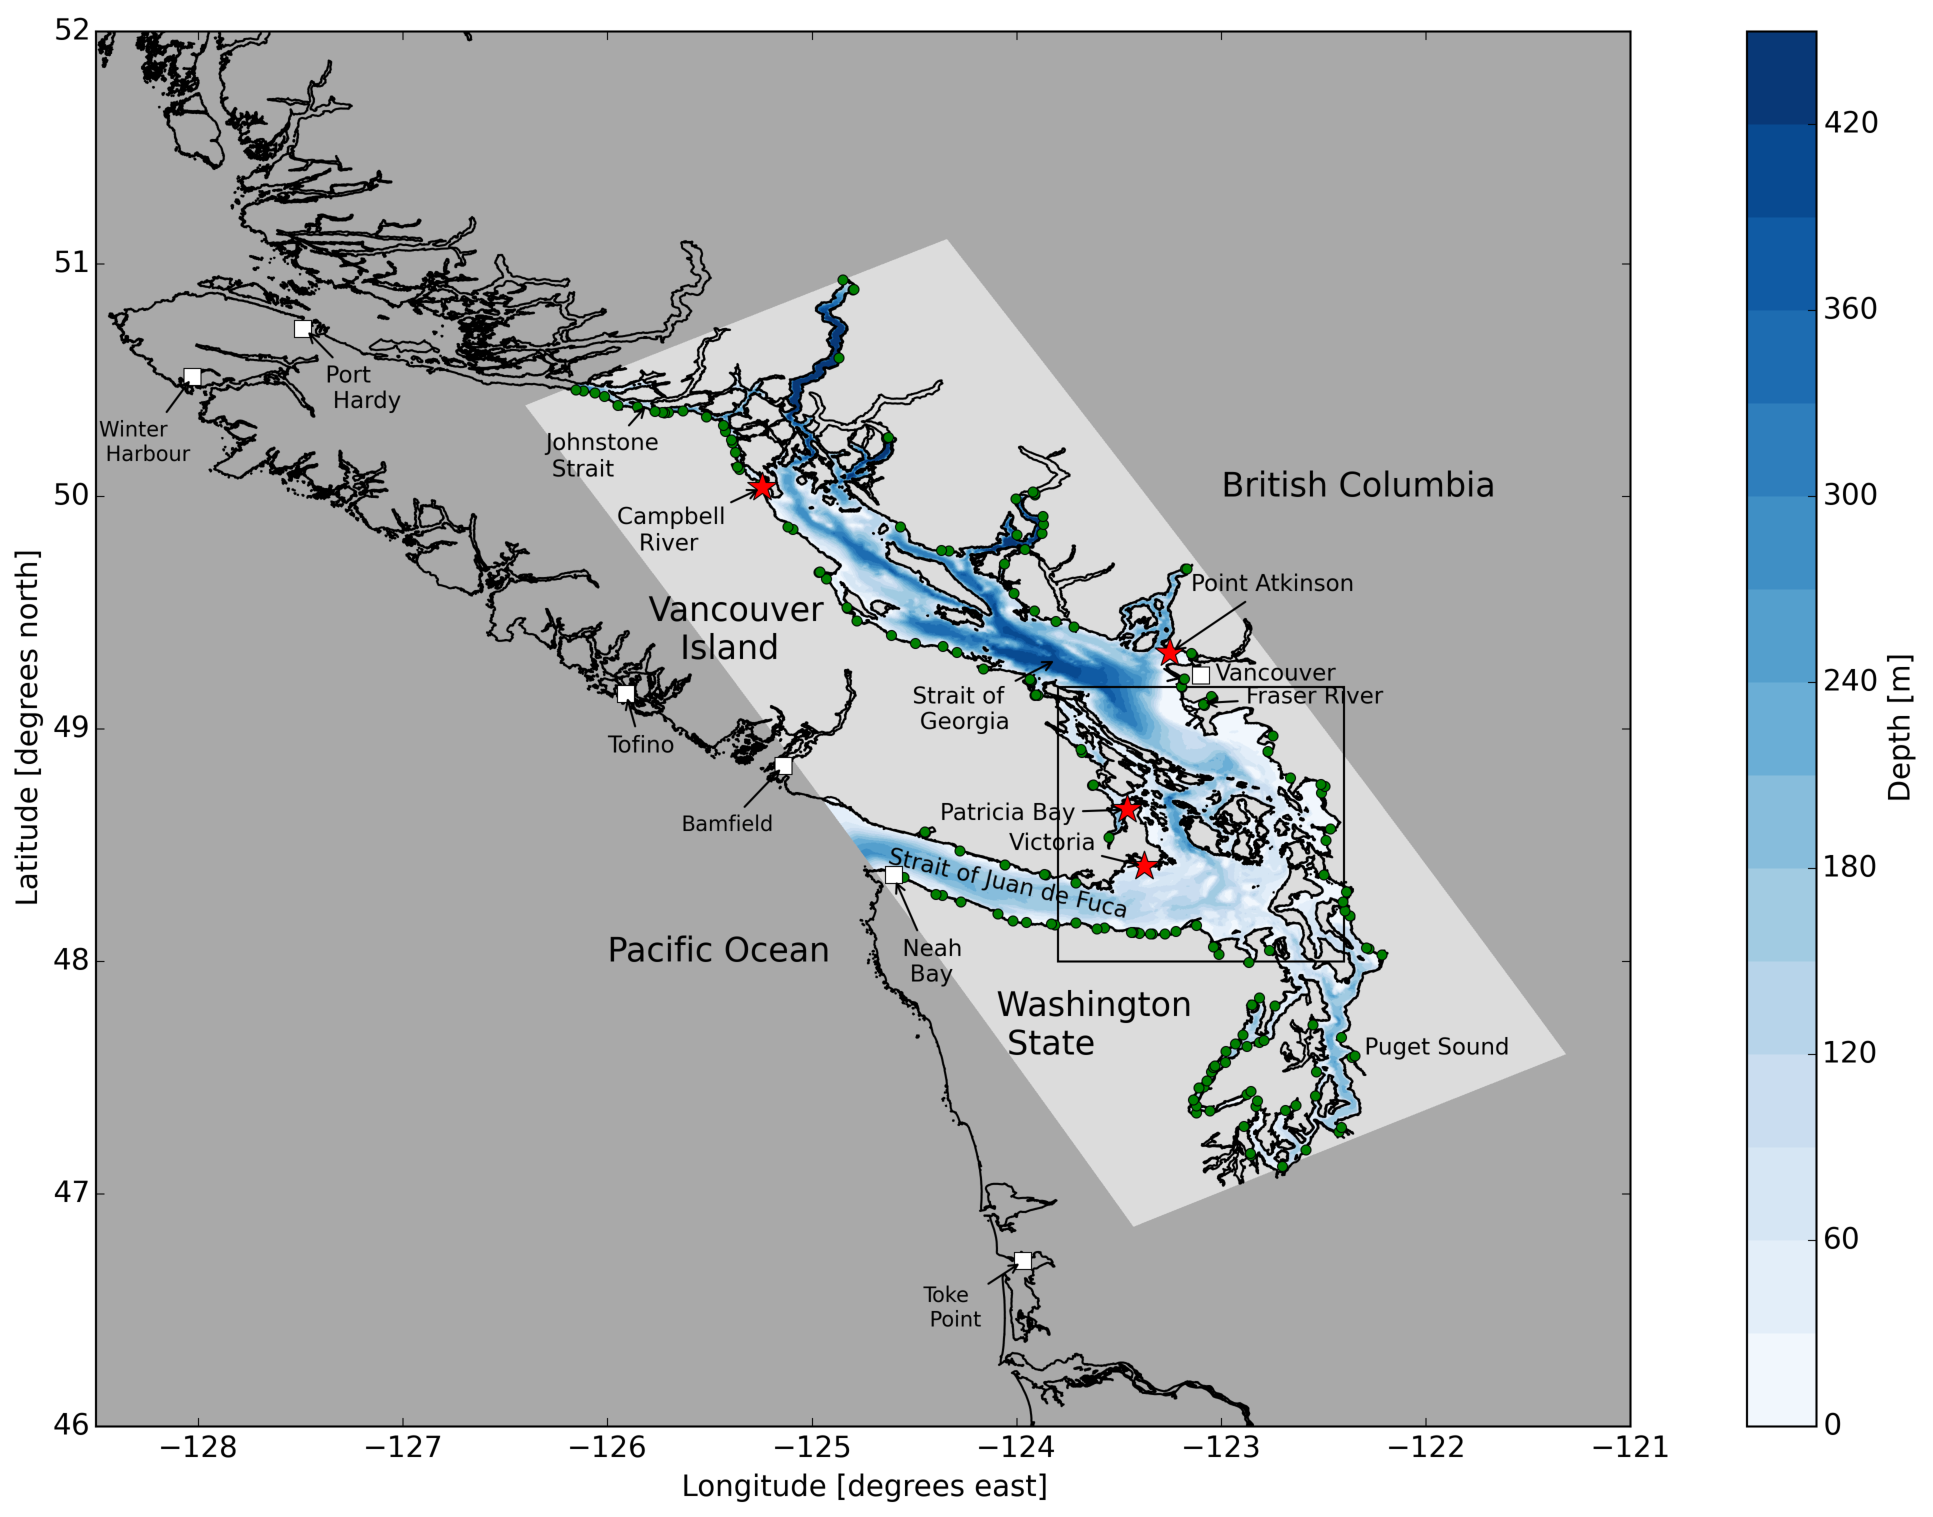
\includegraphics[scale=0.5]{Figures/bathy.pdf}
\caption{Model domain (highlighted area) including bathymetry, rivers (green circles), and storm surge locations of interest  (red stars).}\label{fig:domain}
\end{figure}


The model includes two open boundaries that connect to the Pacific Ocean, the western boundary of the Strait of Juan de Fuca as well as Johnstone Strait at the north, both of which are forced with eight tidal constituents (K$_1$ ,O$_1$, P$_1$, Q$_1$, M$_2$, K$_2$, N$_2$, S$_2$), temperature and salinity climatologies, and the sea surface height anomaly. Tidal heights and currents at grid points along the Juan de Fuca boundary were extracted from Webtide \citep{webtide}, an online web prediction model that provides tidal predictions for the northeast Pacific Ocean based on work by \citet{foreman2000webtide}. The Johnstone Strait boundary was forced with current and elevation tidal harmonics measured and calculated by \citet{thomson1980johnstone} for the major M$_2$ and K$_1$ constituents. Additionally, O$_1$ and S$_2$ elevation harmonics from their measurements were employed. The remaining constituents were extrapolated from Webtide. At the western boundary, the tidal elevation and currents forcing parameters were tuned for a good match with observations at locations within the Strait of Georgia, including Point Atkinson, Gibsons Landing, Winchelsea and Halfmoon Bay. At the northern boundary, the tides were tuned for good matches at Yorke Island and Kelsey Bay. Further details on the tuning are provided in Appendix \ref{sec:appendix}. 

Temperature and salinity at the Juan de Fuca boundary were taken from a weekly climatology which was created from results of a model covering the Salish Sea and the west coast of Vancouver Island \citep{massonfine2012}.  Their results, originally on $s$-levels were interpolated onto $z$-levels and then onto the NEMO horizontal grid to give a two-dimensional forcing that varies with time.  To prepare the climatology all years (1995-2008) were averaged and results, approximately every 15 days, were interpolated to a weekly climatology. The model is relaxed to the forced temperature and salinity over the 10 grid points (about 5 km) closest to the open boundaries, using a flow relaxation scheme \citep{engedahl1995use}. %other references?

Sea surface height anomaly (or remote forcing) was set uniformly across the mouth of Juan de Fuca using values from the Tofino tide gauge \citep{DFOObservations} which is outside of, but close to, the western boundary of the model domain.  A monthly climatology was produced using daily averages from 2000-2010, binning them by month, averaging and setting the yearly mean to zero.  For the storm surge simulations, hourly variations in sea surface height were used.  These values are the Tofino tide gauge values with the tides removed. Tidal predictions were generated with a tidal analysis package called t\_tide \citep{pawlowicz2002classical} using a time series from the year prior to the surge event to avoid over predicted constituents during high surge years. The storm surge simulations also used the sea surface height anomaly from Port Hardy (50.72 $^\circ$ N, 127.49 $^\circ$ W), forced at the northern boundary in Johnstone Strait. The tidal forcing and remote forcing were applied using the NEMO Flather scheme \citep{flather1994storm, madec2012nemo}, a radiation scheme that allows disturbances to propagate out of the domain without reflections off of the open boundary. The barotropic velocity component of the remote forcing was set to zero. At the west, the baroclinic velocities at the boundary were set equal to the values inside the boundary (zero-gradient boundary conditions).  This scheme is not part of core NEMO 3.4 (the version used here).  Zero gradient conditions were chosen because the baroclinic velocity at the mouth of Juan de Fuca is primarily estuarine and thus set by density variations between inside and outside the domain. At the north baroclinic velocities were set to zero. 

At coastal boundaries, the partial slip boundary condition, an approximation to no slip, is used. Partial slip allows one to include the frictional effects of lateral boundaries without the restrictive resolution required to represent the lateral boundary layer under no slip conditions. A lateral eddy viscosity of 20 m$^2$ s$^{-1}$ parametrizes horizontal friction and a lateral eddy diffusivity of 20.5 m$^2$ s$^{-1}$ is used.  Bottom friction is represented by a quadratic law for the bottom momentum flux with drag coefficient $C_D = 5\times 10^{-3}$. Vertical turbulence and mixing is calculated through the $k-\epsilon$ configuration of the generic length scale (GLS) turbulence closure \citep{umlauf2003generic} with background vertical eddy viscosity and diffusivity set to $1\times10^{-4}$ m$^2$ s$^{-1}$ and $1\times10^{-5}$ m$^2$ s$^{-1}$ respectively. Details on the NEMO implementation of the partial slip lateral boundary condition, quadratic bottom friction law, and GLS turbulence closure scheme are provided by \citet{madec2012nemo}.

The ocean surface is forced with momentum and heat fluxes from a 33-km global atmospheric reforecasting model suitable for use in ocean modelling \citep{smith2014new}. Forecasts from the period of 2002-2012 are available. One additional simulation employs the western Canada component of the High Resolution Deterministic Prediction System (HRDPS), a nested 2.5 km resolution atmospheric model provided by Environment Canada \citep{ECModel}. In addition to momentum and heat fluxes, forcing due to the surface atmospheric pressure is also included in the ocean momentum equations \citep{madec2012nemo}. In the open ocean, the surface atmospheric pressure primarily induces an inverse barometer (IB) sea surface height,
\begin{equation}
 \eta_{IB} = -\frac{1}{g\rho_{0}}\left(P_{s}-P_0\right), \label{eq:inverse}
\end{equation}
where $g$ is the acceleration due to gravity, $\rho_{0}$ is a reference density set to 1035 kg m$^{-3}$, $P_{s}$ is the sea level atmospheric pressure from the atmospheric model, and $P_0$ is a reference sea level pressure (set to 101,000 Pa). Since the atmospheric model employs a terrain following vertical coordinate the model surface pressure has been corrected to sea level using \citep{holton1992introduction}
\[ P_s = P_1\left(\gamma\frac{z_1}{T_1} +1 \right)^\frac{g}{\gamma R},\]
where $P_1$ and $T_1$ are the model pressure and temperature at height $z_1$, $R$ is the ideal gas constant, and $\gamma$ is a temperature lapse rate set to 0.0098 K m$^{-1}$. In coastal and shelf seas, the atmospheric pressure forcing can also induce significant non-IB sea surface height, as demonstrated in previous studies of the Hudson Bay and Labrador shelf system \citep{wright1987influence,young1995synoptic}.

River input provides a significant volume of fresh water to the Salish Sea and can influence stratification, circulation, and primary productivity. However, most rivers in the domain are not gauged so parametrizations were required to represent river flow. \citet{morrison2011rivers} provides a method for estimating freshwater runoff in the Salish Sea region based on precipitation. Monthly runoff volumes for each watershed for each year from 1970 to 2012 were acquired from \citet{morrison2011rivers}, as well as monthly averages. Freshwater runoff from each watershed was divided among the rivers in that watershed. The area drained by each river was estimated from Toporama maps by the Atlas of Canada and watershed maps available on the Washington State government website. The watersheds included in our model were Fraser (which represents approximately 44\% of the freshwater input into our domain), Skagit (12\%), East Vancouver Island (North and South) (12\%), Howe (7\%), Bute (7\%), Puget (6\%), Juan de Fuca (5\%), Jervis (4\%) and Toba (3\%). The monthly flow from each river was input as a point source from 0 to 3 metres at the model point closest to the mouth of each river. Incoming water was assumed to be fresh and at surface temperature. A total of 150 rivers were parametrized by this method and their locations are indicated by the green dots in Figure \ref{fig:domain}.

Initial conditions for temperature and salinity came from a CTD cast in the middle Strait of Georgia taken in Sept 2002 \citep{pawlowiczetal2007}. Conditions were initially uniform horizontally and velocity was initialized at zero. The model was spun up for 15.5 months from the initial conditions above, starting Sept 16, 2002, using atmospheric forcing from 2002-2003, climatological temperature and salinity and sea surface height at the boundaries, with tides and climatological river output.  All storm surge runs were started at least three days prior to the event of interest with zero initial velocities and sea surface height and a stratification profile from model spin up. The modelled sea surface height adjusted to forcing in less than one day. 

\section{Tidal Evaluation}\label{sec:model}

The model was initially evaluated qualitatively by comparing patterns of tidal amplitude and phase to results from \citet{foreman1995tidal}, focusing on the major M$_2$ and K$_1$ constituents. For example, the M$_2$ amphidrome around Victoria was reproduced as well as the monotonic increase in $K_1$ amplitude moving northwards along the Strait of Georgia. As the model was reproducing observed tidal patterns, model results were quantitatively evaluated by comparing modelled harmonic constituents to measured harmonic constituents at tidal measuring stations throughout the domain. Comparisons were made using the complex difference ($D$), defined as \citep{foreman1995tidal}:

\begin{equation}
D = [(A_0 \cos g_0 - A_m \cos g_m)^2 + (A_0 \sin g_0 - A_m \sin g_m)^2]^{1/2}
\end{equation}\label{eq:compdiff}
where $A_0$, $A_m$, $g_0$ and $g_m$ are the observed and modelled amplitudes and phases. Figure \ref{fig:tides} compares modelled and observed amplitude, phase, and complex differences for the $M_2$ and $K_1$ tidal constituents for stations along a transect from the Strait of Juan de Fuca through to the Strait of Georgia and Johnstone Strait. Comparisons have been made with data from \citet{foreman1995tidal}, \citet{foreman2004m} and \citet{foreman2012circulation}. Station names and numbers are listed in Table  \ref{tab:comparison} in Appendix \ref{sec:appendix}.

In general, the K$_1$ tidal harmonics are well-represented by the model with complex differences below 5 cm at all stations except Seymour Narrows (station 27). Seymour Narrows is a very constricted region in Johnstone Strait and is not well resolved by the model. As such, the M$_2$ amplitude and phase are also poorly reproduced here. The model's M$_2$ amphidrome, indicated by the drop in amplitude around station 5 (Victoria), is too strong resulting in lower than observed M$_2$ amplitudes in this region. Additionally, the M$_2$ phase errors in the Strait of Juan de Fuca (stations 1-7) are quite large, leading to large complex differences in this region.  However, the match in the Strait of Georgia (stations 10-24) is very good, with complex differences less than 6 cm, in part due to tidal tuning for highly accurate tides in the main region of interest. Details on the tidal tuning procedure are provided in Appendix \ref{sec:appendix}.

%perhaps a table of complex differences at tidal stations similar to Table 1 of Foreman et al (1995)  (such as the one produced by tidetools.calc_diffs_meas_mod) here?
%(would be cool to include the complex differences calculated at the VENUS nodes too)
%perhaps a nice contour map of M2 and K1 amps and phases goes here?
%if it's favourable, we could compare our complex differences to Foreman et al (1995), who got an average of D=3cm for M2 and D=2.5cm for K1

\begin{figure}
\centering
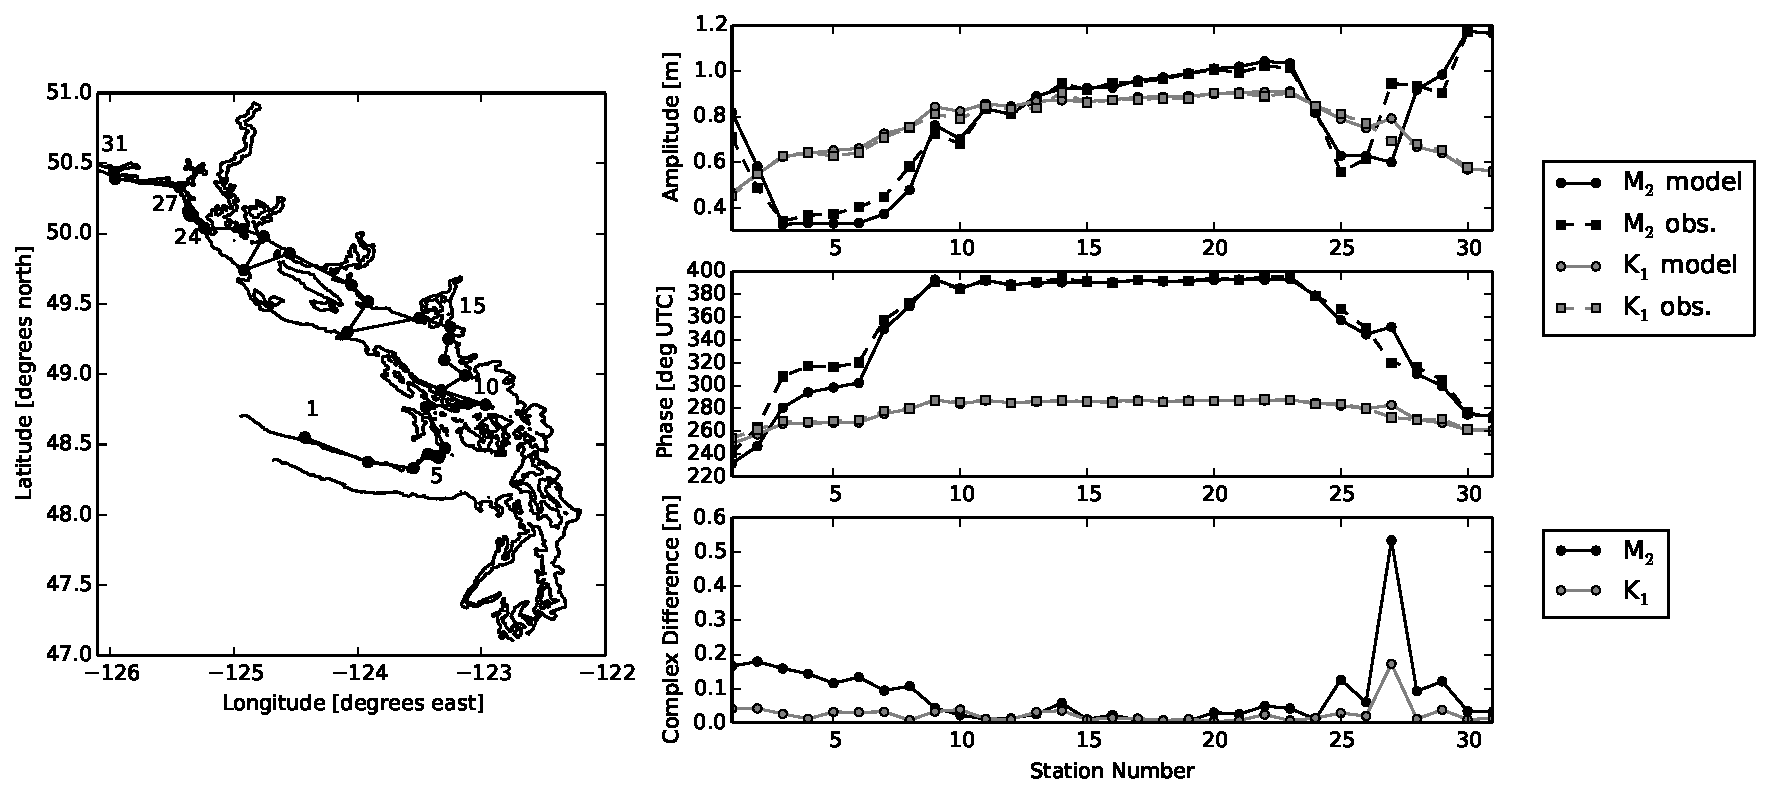
\includegraphics[scale=0.6]{Figures/tides.pdf}
\caption{Evaluation of model tidal amplitude and phases for the M$_2$ and K$_1$ constituents. On the left, a transect through the stations used for comparison. On the right, modelled M$_2$ (black) and K$_1$ (grey) amplitude (top) and phase (middle) compared with observations in the dashed curves of the same colour. The bottom plot displays the M$_2$ and K$_1$ complex differences. Station names and numbers are listed Appendix \ref{sec:appendix} in Table \ref{tab:comparison}.}
\label{fig:tides}
\end{figure}


\section{Storm Surge Hindcasts}\label{sec:storm}
A series of five storm surge hindcasts is presented next. Storm surge simulations were started from rest at least three days prior to the event of interest to allow for adjustment of model currents. Stratification conditions from model spin up at a time close to the event (within five days) were chosen to initialize the temperature and salinity fields. Boundary conditions include atmospheric forcing and fresh water input from rivers at the surface, sea surface height anomaly from observations at the open boundary, and tidal forcing with eight tidal constituents. Forcing the model with only eight tidal constituents leads to an error in modelled sea surface height due to the omission of the next leading order tidal constituents such as J$_1$. Comparisons between full tidal predictions and tidal predictions using eight constituents suggest that this error can approach 40 cm during times of high tidal range, and in particular, during the storm surge season Nov-Feb. As such, storm surge model predictions were corrected by accounting for this error; for each storm surge location of interest, the difference between a full tidal prediction and a tidal prediction with eight constituents is added to the modelled sea surface height. This correction is only applied to the modelled water level and not the modelled residuals. Additionally, since the modelled sea surface height is calculated about a zero reference level, the modelled water level is determined by adding a long term mean sea level at the specified location to the modelled sea surface height. All times are reported in UTC.

Model results have been compared with observations by calculating both the total modelled water level and the modelled residual at four permanent tidal measuring stations: Point Atkinson, Victoria, Patricia Bay, and Campbell River (locations indicated in Figure \ref{fig:domain}). The modelled residual is calculated as the difference in model output between a simulation with all forcing conditions and a simulation forced only with tides and rivers. Water level observations are taken from the Canadian Tides and Water Level Data Archive \citep{DFOObservations} and are used to calculate the observed residual, defined as the observed water level minus tidal predictions. Tidal predictions are calculated using t\_tide \citep{pawlowicz2002classical}, a MATLAB tool that calculates tidal harmonics from a given time series, in this case, from the year prior to the surge event of interest. 

The model's skill is reported through a few statistical measures of the the total water level $\eta$ and the residual $\delta$. First, the mean absolute error ($\bar{e}$), defined as
\begin{equation}
\bar{e} = \text{mean}\left(\left| M - O \right|\right),
\end{equation}
where $M$ and $O$ are the modelled and observed quantities of interest, is a common measure that estimates the average error in the model. Next, a measure comparing the variance of the error to the variance of the observations defined as \citep{thompson2003prediction},
\begin{equation}
\gamma^2 = \frac{\text{var}\left(M-O\right)}{\text{var}\left(O\right)},
\end{equation}
is also calculated. Smaller values of $\gamma^2$ indicate better model skill. This quantity was used by \citet{bernier2006predicting} and \citet{bernier2010tide} in storm surge predictions in Eastern Canada and is calculated here as a point of comparison. A third measure, called the Willmott skill score \citep{willmott1982some}, is also used to assess overall model skill in predicting the water level and residual. This quantity is defined as
\begin{equation}
WS = 1 - \frac{\sum_{i=1}^N \left(M_i - O_i\right)^2}{\sum_{i=1}^N \left(|M_i'| + |O_i'|\right)^2},
\end{equation} 
where $M_i' = M_i-\bar{O}$ and $O_i'=O_i-\bar{O}$ and $\bar{O}$ is the mean of the observations. This score is bounded by zero and one and values close to one indicate good model skill. Since the Willmott skill score is nondimensional, it is an appropriate statistic to report when comparing skills of different variables, in this case, the total water level and the residuals. Since the total water level has a larger variability than the residuals, the $\gamma^2$ measure should be much lower for the total water levels; hence, the Willmott skill score provides an additional point of comparison. These three statistics, along with the mean observed values and mean modelled values (which indicate the model's bias) are reported in Table \ref{tab:statistics} for each hindcast.  

The five hindcast simulations have been used to assess the model's skill and to learn more about how the storm surge propagates through the Salish Sea domain.  First, a general assessment of the model's skill is presented in two hindcasts during Feb 2006 and Nov 2006 in section \ref{sec:hind}.  Second, the contribution to the surge due to several forcing conditions, such as atmospheric forcing and open boundary forcing, has been assessed for the Feb 2006 case in section \ref{sec:factors}. This case is also used to determine the importance of modelling tidal forcing with the surge propagation. Third, the spatial variability of the surge as it propagates through the domain is examined for a Dec 2006 storm surge in section \ref{sec:spatial}. Fourth, a high wind event that did not result in a large surge or flooding for a Nov 2009 case is discussed in section \ref{sec:wind}. Finally, comparisons between hindcasts using high resolution (HRDPS) and low resolution (CGRF) atmospheric forcing is provided for the Dec 2012 case in section \ref{sec:res}. 

\subsection{Example Storm Surge Hindcasts}\label{sec:hind}

A hindcast for a storm surge that occurred on Feb 4, 2006 is presented next. The simulation ran from Feb 1-8, 2006. The model's ability to reproduce this event is demonstrated in Figure \ref{fig:feb2006} which compares observations to corrected model output at Point Atkinson, Victoria, Patricia Bay, and Campbell River. First, the timing of maximum water level matches well between the observations and the model at all four locations, the most significant contribution to high water being from the tides which are generally well-represented by the model. There is good agreement in the water level maximum at both Victoria and Patricia Bay, although it is slightly under predicted at these two locations. The maximum water level at Point Atkinson and Campbell River is slightly over predicted and the error is more significant, but the tidal range is also larger. It is surprising that Victoria and Patricia Bay agree so closely with observations because the M$_2$ tidal amplitudes in the model are known to be too low in this area. When considering the over predicted water levels at Point Atkinson and Campbell River, it is likely that one of the forcing factors is overestimated in this example. 

In general, there is also very good agreement between the observed and modelled residuals (Figure \ref{fig:feb2006}). The most noticeable difference is a 4-6 hour delay in the model's timing of the maximum residual except at Victoria where the maximum residual is in phase with observations. The surge manifests as a broad peak in both the modelled and observed residual leading to a high probability that large residuals coincide with the high tide. As such, it is of minor consequence that the timing of the observed and modelled maximum residual do not match perfectly. 

\begin{figure}
\centering
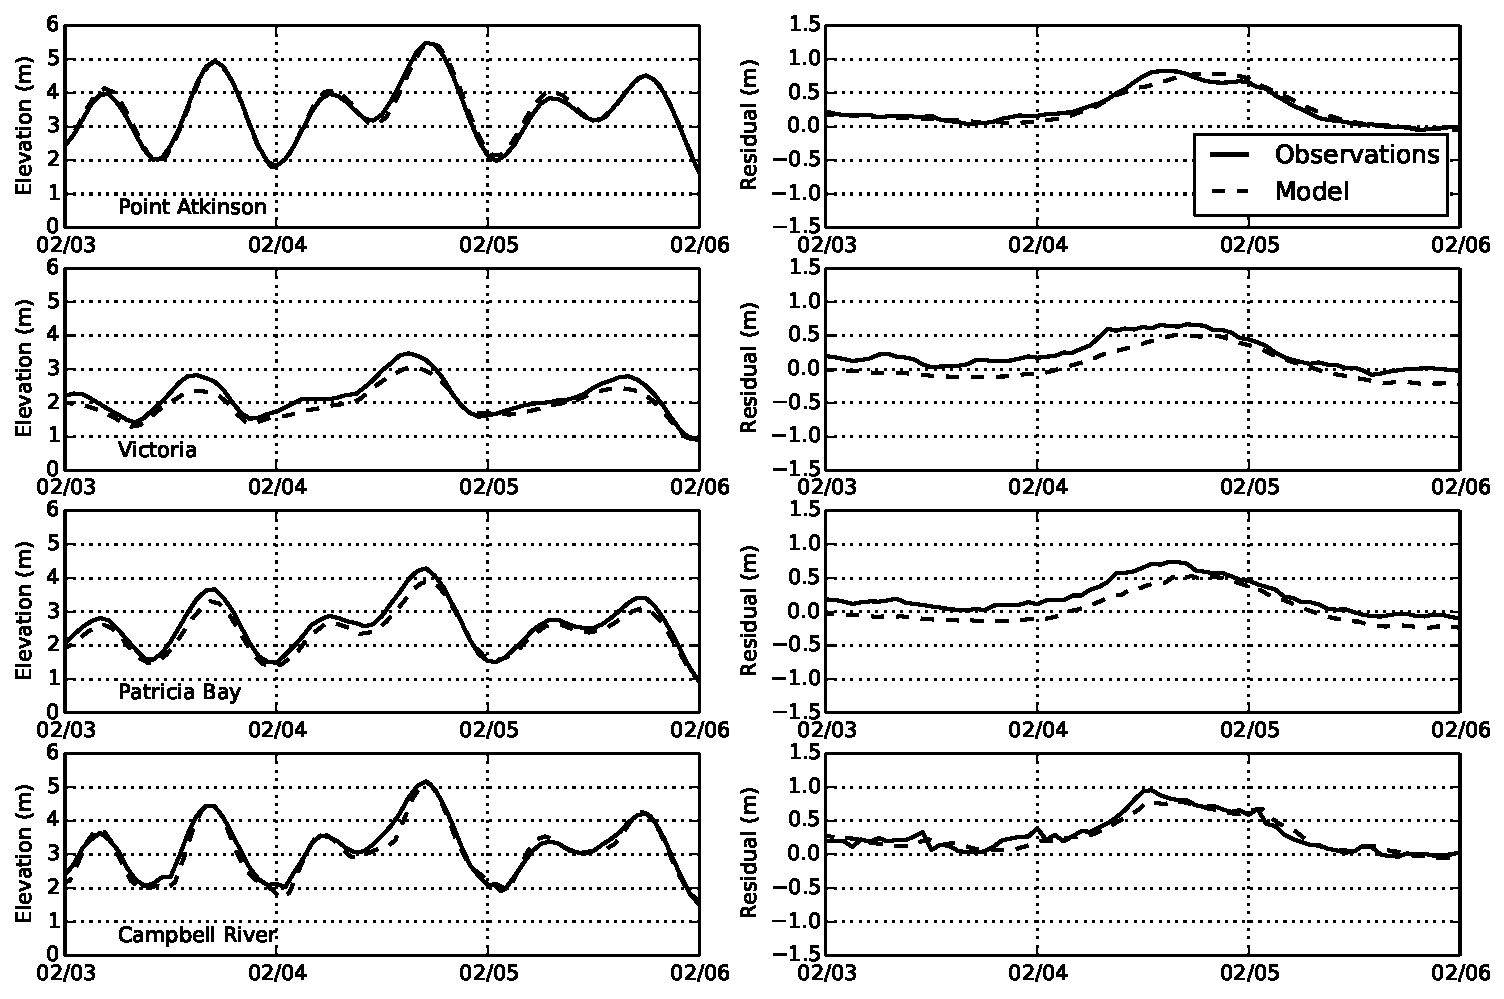
\includegraphics[scale=0.6]{Figures/feb2006.pdf}
\caption{Comparison of observations and model output for the Feb 4, 2006 storm surge. Left: total water level observation (solid) and corrected model (dashed). Right: observed residuals (solid) and modelled residuals (dashed).}
\label{fig:feb2006}
\end{figure}

A more detailed evaluation of the model performance is provided by a group of statistical measures, including the mean absolute error, the observed mean, the modelled mean, $\gamma^2$, and the Willmott skill score for both the water level and residuals (Table \ref{tab:statistics}). The statistics are calculated with hourly output over the three-day period displayed in Figure \ref{fig:feb2006}. The mean absolute error in the water level ranges from 7.6 cm at Victoria to 13.1 cm at Campbell River, whereas, the mean absolute error in the residuals is smaller at all stations; however, this measure does not account for the large variability in water levels due to the tides. A statistic that does take into account this variability is $\gamma^2$ which suggests very good agreement in both the predicted water levels and residuals. Good agreement is also reflected in high Willmott skill scores at all locations. Note that the $\gamma^2$ measures and Willmott skill scores degrade slightly for the residuals, likely because the well-tuned tidal signal dominates the water level predictions.

\begin{table}[h]
\centering 
\tbl{Evaluation of model performance for all hindcasts presented. Mean absolute error ($\bar{e}$), observed mean (subscript o), modelled mean (subscript m), $\gamma^2$, and the Willmott skill score ($WS$) are provided for water level predictions ($\eta$) and residuals ($\delta$). Statistics are calculated over the time period displayed in each simulation's corresponding figure (three or four days). For the Nov 2006 case, the statistics were calculated over a three day period. The average values were calculated over all of the hindcasts, excluding the Dec 2012 HRDPS simulation. } 
{\begin{tabular}{|l |c c c c c | c c c c c|} 
\hline 
& \multicolumn{5}{|c|}{Water Level ($\eta$)}        & \multicolumn{5}{|c|}{Residual ($\delta$)} \\ 
\hline 
Location       & $\bar{e}$ (cm) & $\bar{\eta_{o}}$ (m) & $\bar{\eta_{m}}$ (m) & $\gamma^2$ & $WS$   & $\bar{e}$ (cm) & $\bar{\delta_{o}}$ (m) & $\bar{\delta_{m}}$ (m) & $\gamma^2$ & $WS$ \\
\hline 
Feb 2006& & & & & & & & & &\\ 
Point Atkinson & 11.6& 3.458& 3.558& 0.012& 0.994& 5.5& 0.318& 0.33& 0.058& 0.985\\
Victoria       & 8.2& 2.182& 2.205& 0.035& 0.99& 5.3& 0.276& 0.298& 0.075& 0.979\\
Patricia Bay   & 10.4& 2.601& 2.678& 0.025& 0.99& 5.5& 0.275& 0.298& 0.066& 0.981\\
Campbell River & 12.2& 3.202& 3.235& 0.034& 0.991& 7.0& 0.27& 0.317& 0.066& 0.973\\
\hline
Nov 2006& & & & & & & & & & \\
Point Atkinson & 10.2& 3.422& 3.499& 0.026& 0.99& 6.7& 0.32& 0.305& 0.128& 0.96\\
Victoria       & 7.8& 2.158& 2.182& 0.065& 0.982& 4.7& 0.246& 0.26& 0.134& 0.961\\
Patricia Bay   & 9.4& 2.565& 2.634& 0.043& 0.983& 5.9& 0.258& 0.261& 0.152& 0.953\\
Campbell River & 9.9& 3.201& 3.243& 0.032& 0.991& 6.3& 0.29& 0.293& 0.153& 0.951\\
\hline
Dec 2006& & & & & & & & & & \\
Point Atkinson & 12.9& 3.452& 3.531& 0.028& 0.99& 10.0& 0.336& 0.33& 0.272& 0.895\\
Victoria       & 8.1& 2.229& 2.226& 0.046& 0.988& 7.2& 0.306& 0.3& 0.227& 0.916\\
Patricia Bay   & 10.2& 2.628& 2.674& 0.035& 0.989& 8.8& 0.308& 0.293& 0.255& 0.896\\
Campbell River & 11.3& 3.234& 3.265& 0.034& 0.991& 8.2& 0.311& 0.304& 0.235& 0.912\\
\hline
Nov 2009& & & & & & & & & & \\
Point Atkinson & 14.5& 3.426& 3.55& 0.01& 0.995& 8.3& 0.344& 0.397& 0.204& 0.897\\
Victoria       & 10.9& 2.249& 2.24& 0.029& 0.992& 4.4& 0.365& 0.361& 0.201& 0.933\\
Patricia Bay   & 12.0& 2.589& 2.685& 0.021& 0.991& 7.4& 0.307& 0.356& 0.216& 0.894\\
Campbell River & 11.6& 3.219& 3.247& 0.016& 0.996& 6.9& 0.341& 0.38& 0.188& 0.915\\
\hline
Dec 2012-CGRF& & & & & & & & & & \\
Point Atkinson & 11.0& 3.362& 3.432& 0.007& 0.997& 5.7& 0.274& 0.273& 0.219& 0.929\\
Victoria       & 12.9& 2.146& 2.111& 0.036& 0.99& 4.7& 0.282& 0.256& 0.175& 0.934\\
Patricia Bay   & 12.8& 2.551& 2.571& 0.024& 0.993& 5.2& 0.275& 0.255& 0.185& 0.934\\
Campbell River & 12.1& 3.064& 3.106& 0.013& 0.996& 8.4& 0.188& 0.263& 0.216& 0.849\\
\hline
Dec 2012-HRDPS& & &  &  &  &  &  &  &  &  \\
Point Atkinson &  10.5&  3.362&  3.42&  0.007&  0.998&  6.2&  0.274&  0.26&  0.231&  0.921\\
Victoria       &  12.6&  2.146&  2.113&  0.035&  0.99&  4.6&  0.282&  0.258&  0.171&  0.937\\
Patricia Bay   &  12.6& 2.551& 2.575& 0.024& 0.993& 5.0& 0.275& 0.26& 0.175& 0.94\\
Campbell River & 12.1& 3.064& 3.104& 0.014& 0.996& 8.1& 0.188& 0.26& 0.218& 0.854\\
\hline
\hline
Averages& & & & & & & & & & \\
Point Atkinson & 11.6&	3.401&	3.483&	0.013&	0.995&	6.7&	0.302&	0.307	&0.192	&0.932\\
Victoria       &10.8&	2.175	&2.162	&0.04	&0.989	&5.1	&0.29	&0.28&	0.167&	0.94\\
Patricia Bay   &11.6&	2.573&	2.619&	0.028&	0.991&	6.0&	0.281&	0.279&	0.179&	0.932\\
Campbell River & 11.6&	3.139&	3.177&	0.021&	0.994&	7.8&	0.246&	0.293&	0.188&	0.893\\
\hline
\end{tabular}}
\label{tab:statistics}
\end{table} 
%anything else to include? statistics calculated in Feb 2006 -paper production.ipynb and saved in statistics_feb2006.CV 
%I also have standard deviations, correlations, ...
\begin{table}[h]
\centering 
\tbl{{\color{red}Summary of maximum water level, maximum surge amplitude and model delay for all simulations. The model time delay is the number of hours between the maximum in the observations and the maximum in the model. A negative number means the model's maximum was later than the observations. Values calucated over the same periods discusses in Table \ref{tab:statistics}. } }
{\begin{tabular}{|l |c c c | c c c|} 
\hline 
& \multicolumn{3}{|c|}{Water Level ($\eta$)}        & \multicolumn{3}{|c|}{Residual ($\delta$)} \\ 
\hline 
Location       & Max obs (m) & Max mod (m) & Delay (hours) &Max obs (m) & Max mod (m) & Delay (hours) \\
\hline
Feb 2006&  &  &  &  &  & \\
Point Atkinson  & 5.460 & 5.588 & 0 & 0.844 & 0.841 & -3\\
Victoria        & 3.440 & 3.415 & -1 & 0.700 & 0.745 & 1\\
Patricia Bay    & 4.250 & 4.179 & -1 & 0.781 & 0.773 & -2\\
Campbell River  & 5.100 & 5.170 & -1 & 0.876 & 0.815 & -5\\
\hline
Nov 2006 &  &  &  &  &  & \\
Point Atkinson  & 5.010 & 5.040 & 0 & 0.880 & 0.725 & 1\\
Victoria        & 2.995 & 2.968 & 1 & 0.664 & 0.563 & 5\\
Patricia Bay    & 3.840 & 3.743 & 0 & 0.709 & 0.607 & 2\\
Campbell River  & 4.750 & 4.739 & 0 & 0.709 & 0.666 & -1\\
\hline
Dec 2006 &  &  &  &  &  & \\
Point Atkinson  & 4.565 & 4.654 & 0 & 0.944 & 0.699 & 0\\
Victoria        & 2.965 & 3.005 & -1 & 0.737 & 0.580 & 1\\
Patricia Bay    & 3.505 & 3.480 & 0 & 0.859 & 0.613 & 1\\
Campbell River  & 4.295 & 4.389 & -1 & 0.823 & 0.626 & 0\\
\hline
Nov 2009 &  &  &  &  &  & \\
Point Atkinson  & 5.150 & 5.272 & 0 & 0.699 & 0.587 & -7\\
Victoria        & 3.195 & 3.144 & -4 & 0.718 & 0.540 & -8\\
Patricia Bay    & 3.985 & 3.902 & 0 & 0.637 & 0.541 & -8\\
Campbell River  & 4.680 & 4.782 & 0 & 0.664 & 0.588 & -1\\
\hline
Dec 2012-CRGF &  &  &  &  &  & \\
Point Atkinson  & 5.345 & 5.416 & 0 & 0.663 & 0.555 & -4\\
Victoria        & 3.145 & 3.117 & 0 & 0.663 & 0.518 & -4\\
Patricia Bay    & 4.115 & 3.975 & 0 & 0.632 & 0.533 & -4\\
Campbell River  & 4.805 & 4.900 & 0 & 0.578 & 0.507 & -6\\
\hline
Dec 2012-HRDPS &  &  &  &  &  & \\
Point Atkinson  & 5.345 & 5.414 & 0 & 0.663 & 0.555 & -4\\
Victoria        & 3.145 & 3.123 & 0 & 0.663 & 0.518 & -4\\
Patricia Bay    & 4.115 & 3.984 & 0 & 0.632 & 0.533 & -4\\
Campbell River  & 4.805 & 4.905 & 0 & 0.578 & 0.511 & -6\\
\hline
\hline
Averages  &  &  &  &  &  & \\
Point Atkinson  & 5.196 & 5.277 & 0  & 0.752 & 0.634 & -3.125\\
Victoria        & 3.147 & 3.125 & -0.625 & 0.684 & 0.563 & -2.125\\
Patricia Bay    & 4.005 & 3.901 & -0.125 & 0.689 & 0.584 & -2.875\\
Campbell River  & 4.756 & 4.835 & -0.250 & 0.673 & 0.590 & -3.875\\ 
\hline 
\end{tabular}}
\label{tab:peak}
\end{table}

An additional storm surge hindcast for a Nov 16, 2006 storm surge is provided as another means of assessing model performance and is mentioned briefly here. The model performs reasonably well in this hindcast; Willmott skill scores are greater than 0.94 (Table \ref{tab:statistics}).  Further, the $\gamma^2$ statistic suggests that the standard deviation of the error in the modelled residuals is about 40\% ($\sqrt{0.16}$) of the standard deviation of the observed residuals. The best match in maximum surge occurred at Campbell River with a 6.2 cm underestimate by the model. The timing of the maximum surge at Campbell River was identical with observations and too early at the other the stations. 


\subsection{Factors Contributing to Storm Surges}\label{sec:factors}

Next, an assessment of the factors that are most important in the storm surge forcing conditions is presented for the Feb 2006 storm surge (Figure \ref{fig:factors}). Several simulations were done: First, a simulation with all the forcing conditions, including tides, local atmospheric forcing (both local winds and local atmospheric pressure), and sea surface height anomaly at the open boundary (also called remote forcing) in the black curve. Second, a simulation with all forcing except the local atmospheric forcing in the dashed green curve. Third, a simulation with all forcing except the remote forcing in the red curve. Fourth, a simulation with only tides and local wind forcing, that is, excluding remote forcing and local atmospheric pressure forcing in the dashed blue curve. Comparisons between these simulations indicate the relative importance of the remote forcing, the local wind forcing, and the local atmospheric pressure forcing. Finally, a simulation without tidal forcing was performed to study the importance of the tide-surge interaction (Figure \ref{fig:tidesurge}). Contributions due to stratification and bathymetric resolution will be left to a future study. 

First, it is clear that remote forcing at the open boundary contributes most significantly to the surge at each of these locations (Figure \ref{fig:factors}). When the remote forcing is not included as a forcing condition, the surge drops from a maximum 82 cm to 11 cm at Point Atkinson and its maximum occurs eight hours later.  A similar drop in the maximum surge and delay in timing of the maximum surge is observed at the other locations.  When local atmospheric forcing is neglected, almost all of the surge amplitude is accounted for in the remote forcing.

%Local winds
The contribution to the surge due to local atmospheric forcing is small and appears to be geographically dependent, most likely due to the effects of the local winds. Removal of the local atmospheric forcing leads to a drop of about 2.5 cm in the maximum surge at Point Atkinson and 2.3 cm at Campbell River. By contrast, the surge amplitude increases by 4.8 cm at Victoria and 3.6 cm at Patricia Bay. The southeasterly winds over the Strait of Georgia could be acting to push water away from the southern tip of Vancouver Island, resulting in a slight decrease in the surge amplitude at Victoria and Patricia Bay when wind effects are included in the model. A simulation with only tides and local wind forcing produces a surge of 7.8~cm at Point Atkinson, a small fraction of the total observed surge, and only centimetres at the other locations.  Note that this wind-induced surge occurs well after the peak surge occurred in both the observations and simulations with full forcing.

A simple steady state argument balancing the wind stress with the pressure gradient can be used to calculate the slope of the sea surface in a body of water with a constant depth $D$ \citep{pugh2004changing}: 
\begin{equation}
\text{slope} = \frac{C\rho_{air}U^2}{g\rho D},
\end{equation}
where $C$ is the coefficient of friction, $\rho_{air}$ is the density of air, $g$ is the acceleration due to gravity, $U$ is the wind speed, and $\rho$ is the density of water. Given  $C=10^{-3}$, $\rho_{air}=1.23$ kg m$^{-3}$, $\rho= 1035$  kg m$^{-3}$, wind speed $U=20$ m s$^{-1}$, and depth $D=100$ m, the slope of the sea surface is approximately $5\times10^{-7}$. At Point Atkinson, a westerly wind can act over a small distance of approximately 50 km, giving a sea surface elevation on the order of centimetres in agreement with the model findings. Since the Strait of Georgia is not a constant depth and is up to 400 m deep, this calculation is only an approximation. Choosing a larger depth would result in an even smaller estimate for the sea surface elevation caused by wind stresses. Further, northwesterly winds would induce the largest elevations at Point Atkinson due to the large distance over which the winds can act. 

%local pressure
Next, the surge amplitude decreases by a few centimetres at all four locations if local atmospheric pressure is not included in the surface forcing. This drop is smaller than the IB sea level change calculated by equation (\ref{eq:inverse}), approximately 1 cm rise in sea level associated with 1 hPa drop in atmospheric pressure. In this event, the pressure at the Vancouver International Airport dropped to about 99 000 Pa \citep{ECClimateArchive}, corresponding to a 20 cm rise in sea level. This magnitude is in line with the findings of \citet{murty1995storm} that the IB contributes up to $^1/_3$ of the total surge amplitude. In our model, including the influence of remote atmospheric pressure forcing (in the sea level at the open boundary) produces realistic surge amplitudes compared with the runs only including local atmospheric forcing. Our results suggest that the local atmospheric pressure generates a sea level change that is smaller than the IB response. This is related to the small spatial scale of the model domain.   

These comparisons point to the importance of including, as a forcing condition at the open boundary, the surge entering the domain from the Pacific Ocean. Storms travelling over the Pacific Ocean towards the west coast of the northern United States and Canada can induce elevated sea levels along the coastline which then enter the Salish Sea system through the Strait of Juan de Fuca. Previous simulations by \citet{murty1995storm} suggest that the surge entering the system through the Strait of Juan de Fuca contribute most significantly to storm surges in this domain, consistent with the results of the present study.  

\begin{figure}
\centering
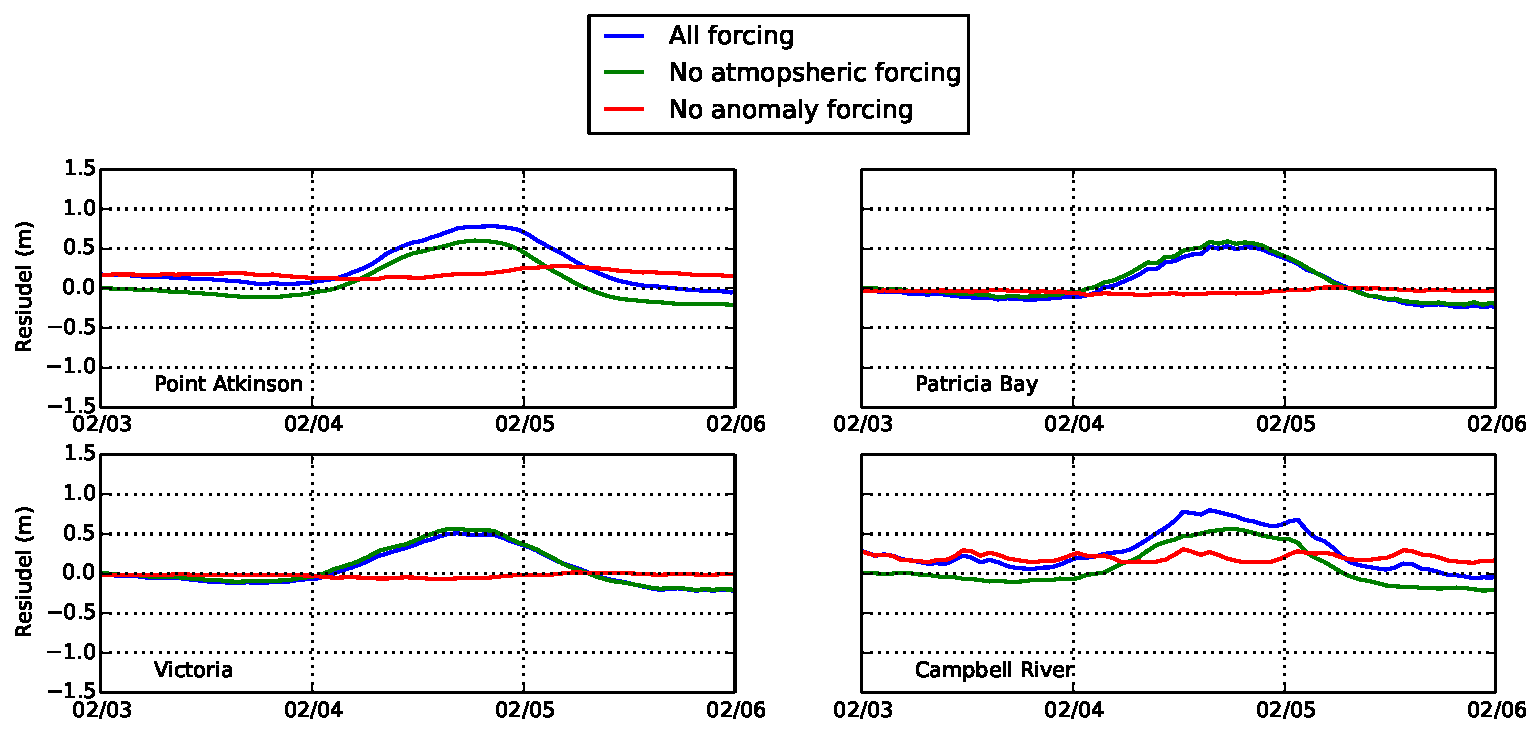
\includegraphics[scale=0.6]{Figures/feb2006_factors.pdf}
\caption{Comparison of the modelled residual for four simulations in Feb 2006: A simulation with all forcing (solid black), a simulation without local atmospheric forcing (dashed green), a simulation without remote forcing (solid red), and a simulation with only tides and local wind forcing, i.e.\ no remote forcing or local atmospheric pressure (dashed blue). }
\label{fig:factors}
\end{figure}

Next, an assessment of the importance of including the tide-surge interaction, which is important in shallow regions due to nonlinear effects and bottom friction \citep{bernier2007tide}, is presented for this hindcast (Figure \ref{fig:tidesurge}). The most significant differences occur at Point Atkinson where the maximum of the surge-only case is 8.7 cm higher than maximum modelled residual, about 10\% of the total surge amplitude.  In contrast, the tide-surge interaction at Victoria is hardly noticeable. Indeed, a spatial map of the difference between the modelled residual and surge-only simulation (Figure \ref{fig:tidesurge_spatial}) indicates that the tide-surge interaction is more pronounced north of the San Juan and Gulf Islands. The passages between these islands are known for vigorous tidal mixing, which may have a nonlinear effect on the surge propagation. However, the effect is a relatively small overestimate of the surge elevation and no changes to the timing of the surge. So, in operational settings, performing a surge-only simulation and adding the predicted tides \textit{a posteriori} could be more computationally efficient with only a small decrease in the accuracy of the prediction. 

\begin{figure}
\centering
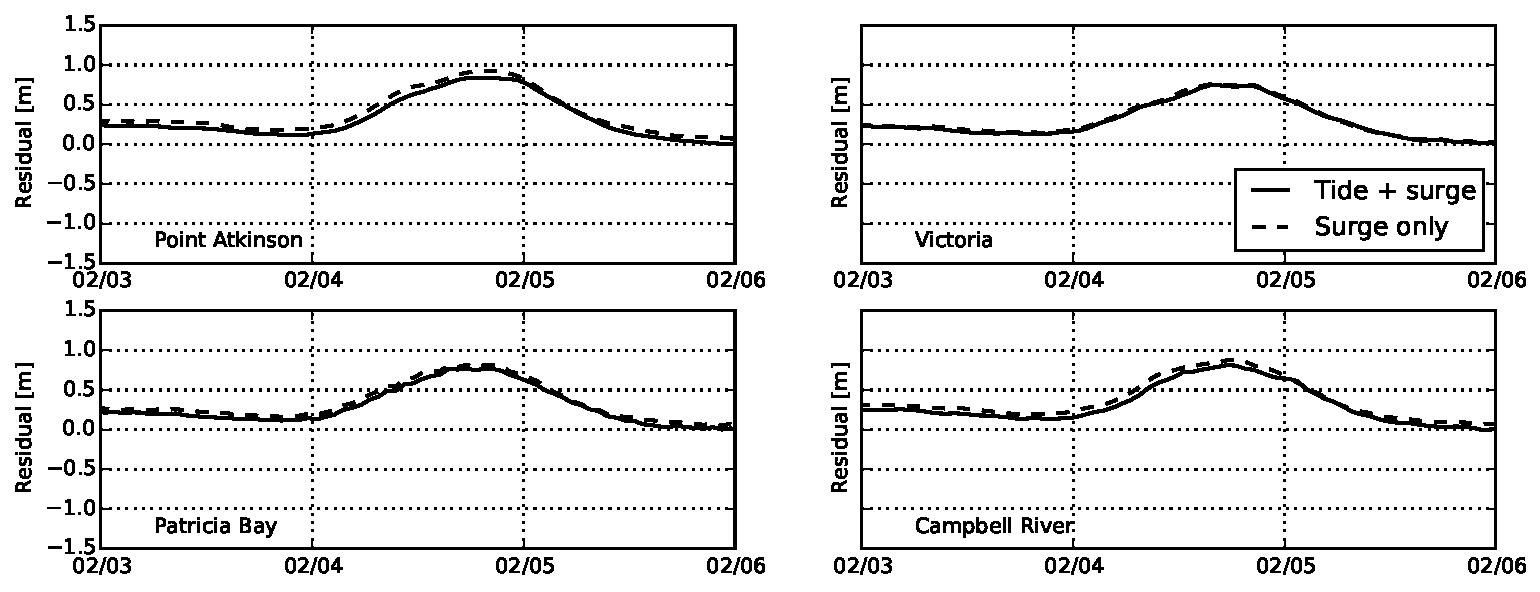
\includegraphics[scale=0.6]{Figures/feb2006_tidesurge.pdf}
\caption{Modelled residuals (solid) compared with a simulation of the surge propagation without tidal forcing (dashed) for the Feb 2006 hindcast. }
\label{fig:tidesurge}
\end{figure}

\begin{figure}
\centering
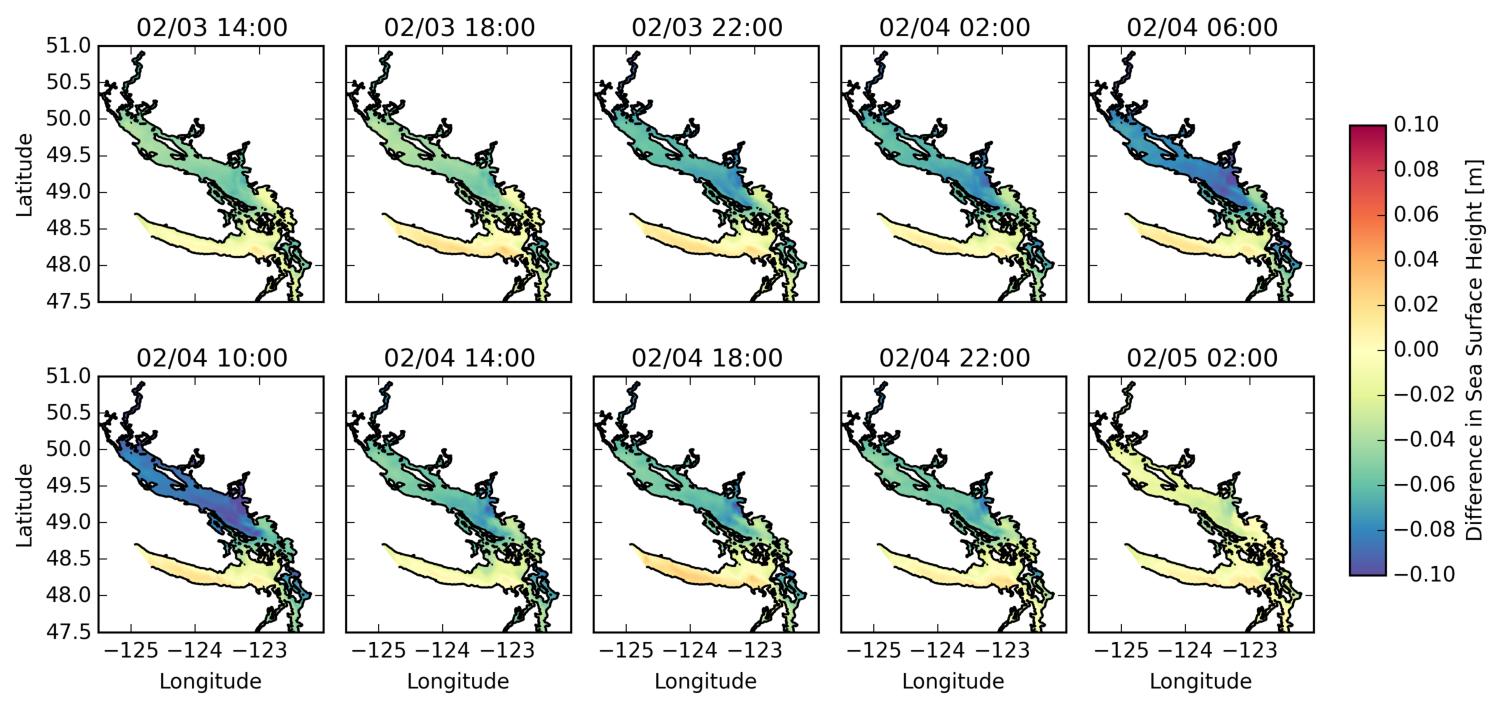
\includegraphics[scale=0.6]{Figures/feb2006_tidesurge_spatial.pdf}
\caption{Spatial dependency of tide-surge interaction in Feb 2006 hindcast. Difference in sea surface height between simulations with tidal forcing and without tidal forcing. Each plot is an average over 4 hours. }
\label{fig:tidesurge_spatial}
\end{figure}


\subsection{Spatial Extent of Surge}\label{sec:spatial}
A major wind storm on Dec 15, 2006 is hindcasted next. Although the storm was very strong (gusts over 120 km hr$^{-1}$) and the observed residual at Point Atkinson reached 84 cm, this event did not coincide with high tide and so no significant or reported flooding occurred in the Vancouver area \citep{forseth2006adaptation}. Because of the high winds, this event has been used to examine the propagation of the surge throughout the domain and spatial variations in the surge amplitude. First, an assessment of the accuracy of the hindcast is provided. 

Modelled residuals are generally too low in this hindcast (Figure \ref{fig:dec2006}), however, the timing of the surge agrees well. All Willmott skill scores rank above 0.88 and the $\gamma^2$ measure also indicates good agreement between model and observations (Table \ref{tab:statistics}). The $\gamma^2$ measure suggests that the standard deviation of the error in the modelled residuals is roughly half of the standard deviation of the observed residuals. Note that the performance has degraded when compared to the Feb 2006 and Nov 2006 cases. This could be due to a number of factors. First, the very large wind speeds observed during this storm are significantly underrepresented by the atmospheric model leading to lower wind stress and less piling of water against the coast. Second, the anomaly forcing at the open boundaries could be too low. The observed residual at Tofino, BC (a point nearby but outside of the domain) is up to 10 cm lower than the observed residual at Neah Bay, WA (a point nearby but inside of the domain). Since the storm surge is less sensitive to wind forcing at the surface than anomaly forcing at the open boundaries, the latter is likely the cause. 

\begin{figure}
\centering
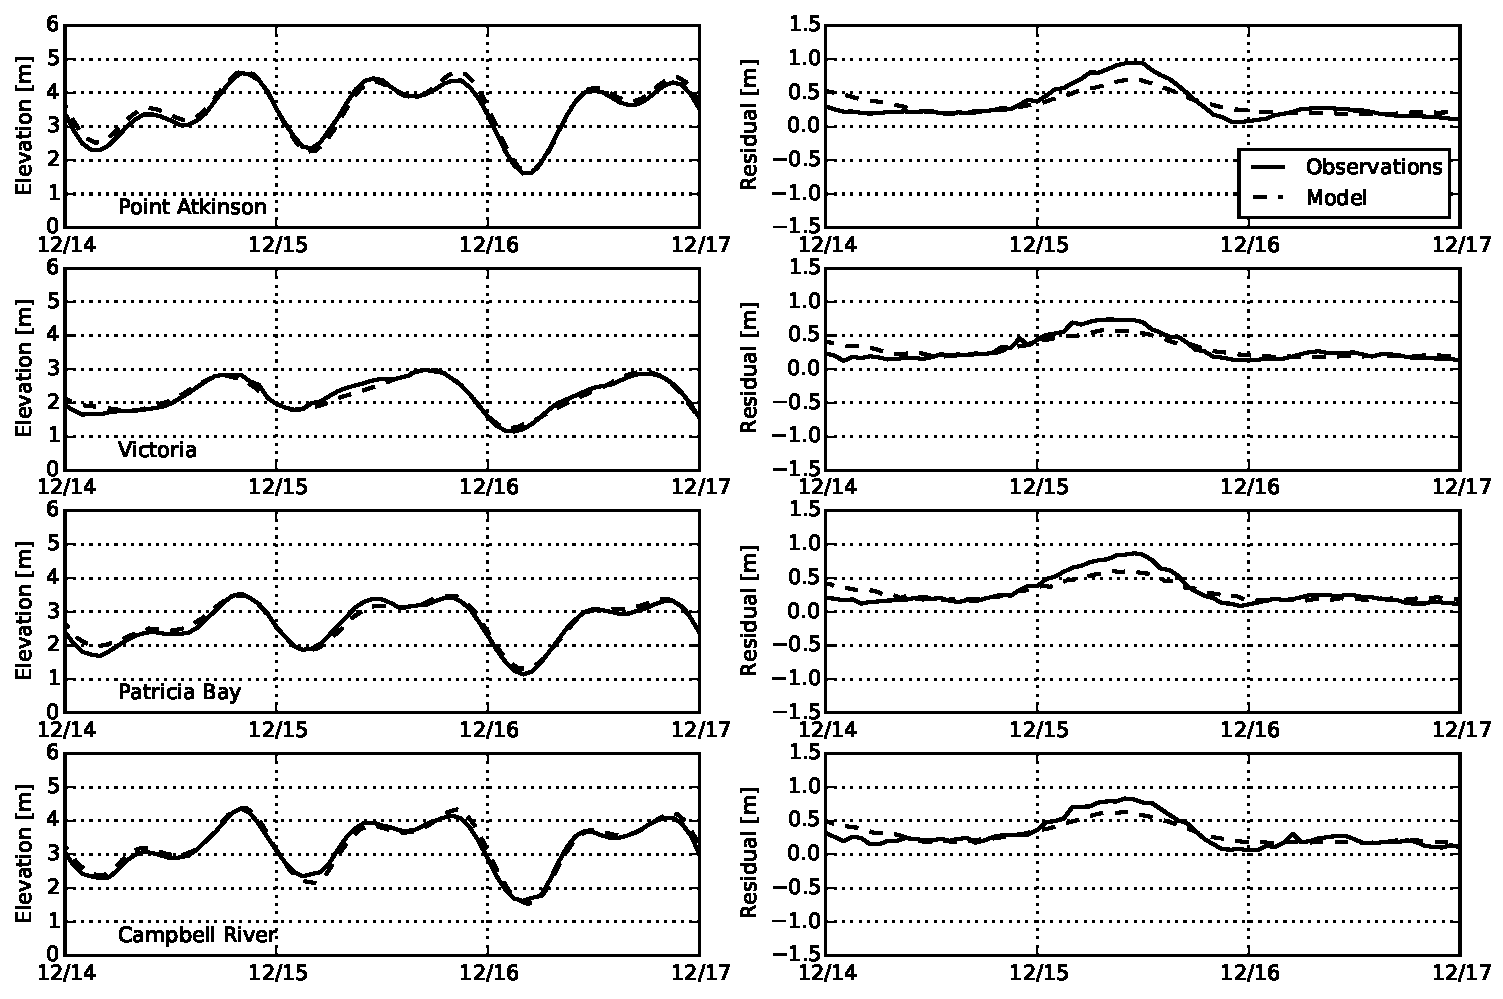
\includegraphics[scale=0.6]{Figures/dec2006.pdf}
\caption{Comparison of observed and modelled water level and residuals during the Dec 15, 2006 storm surge simulation. }
\label{fig:dec2006}
\end{figure}

The evolution and spatial distribution of the surge is highlighted in Figure \ref{fig:spatial} where the modelled residual is plotted every hour beginning on Dec 15 at 05:30 UTC through to Dec 15 at 14:30 UTC. The surge enters the system from the Strait of Juan de Fuca, peaking between Dec 15 at 9:30 UTC and Dec 15 at 11:30 UTC and then begins to subside throughout the entire domain. Notably, the Strait of Georgia experiences the largest surge values, upwards of 60 cm, whereas the Juan de Fuca region experiences a maximum surge around 45 cm. Additionally, the coastal areas on the mainland side of the Strait of Georgia experience slightly higher surges ($\sim$10 cm) than the Vancouver Island side, likely due to the southerly wind in the atmospheric model pushing water against the mainland coast. At about 11:30 UTC, the winds at Point Atkinson switch to northwesterly and then westerly, further amplifying the surge along the mainland coast. 

\begin{figure}
\centering
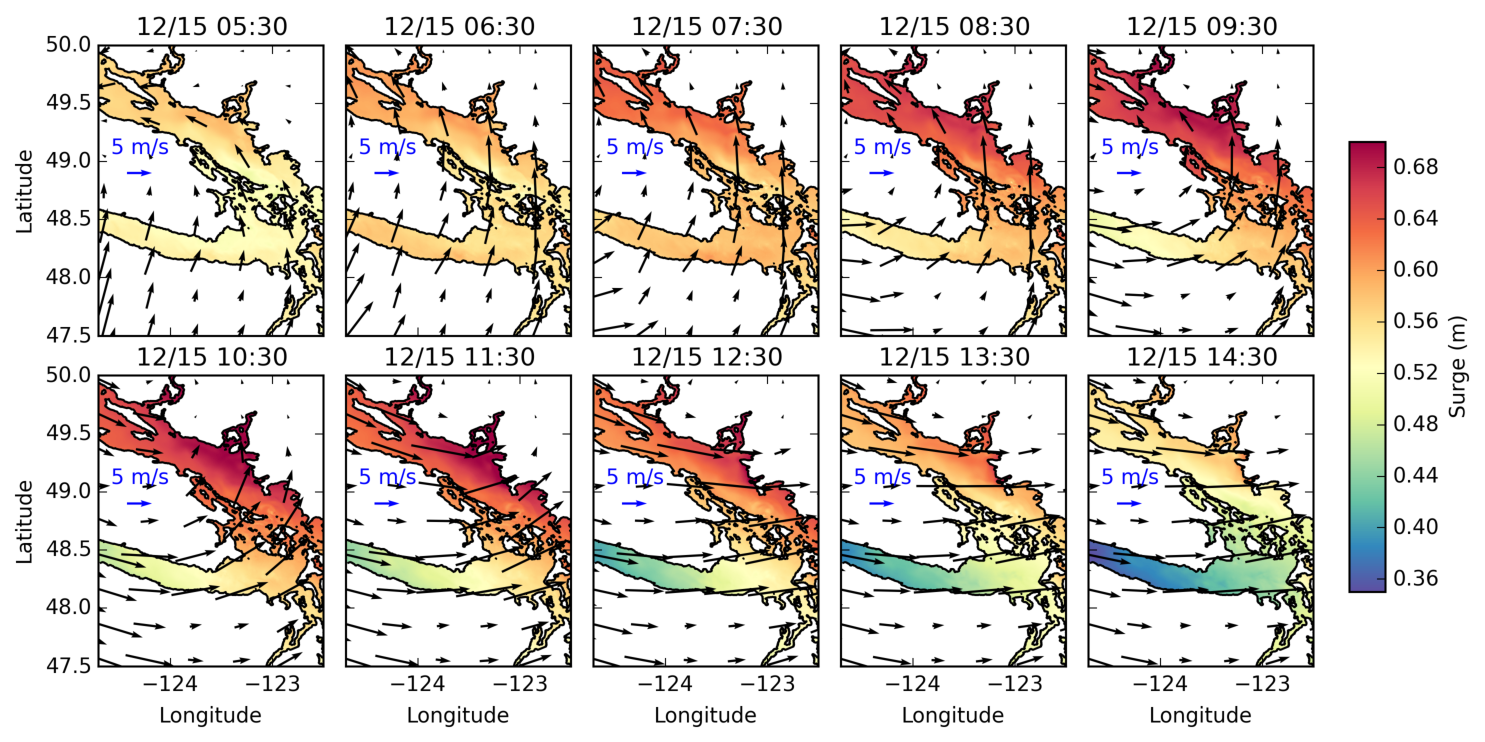
\includegraphics[scale=0.6]{Figures/dec2006_spatial.pdf}
\caption{Propagation of the storm surge on Dec 15, 2006. Modelled residual every hour starting on Dec 15 at 05:30 UTC. Time advances from top left to bottom right. Wind vectors from the atmospheric forcing are overlaid in black.}
\label{fig:spatial}
\end{figure}

In a simulation without atmospheric forcing, the surge amplitude across the Strait of Georgia is uniform with no pronounced difference between the mainland side and Vancouver Island side (Figure \ref{fig:spatial_sshonly}). While the surge entering the domain from the Pacific Ocean is the leading order contribution, the winds may induce localized changes to the surge amplitude. Interestingly, the winds over the Strait of Juan de Fuca cause a decrease in surge amplitude in this region as the winds are acting to push the water towards the mainland.  {\color{red} Even without atmospheric forcing, there is still a significant difference in surge amplitude between the Strait of Georgia and the Strait of Juan de Fuca, perhaps the incoming surge wave is partially reflected from the mainland coast in the Strait of Georgia}. 

\begin{figure}
\centering
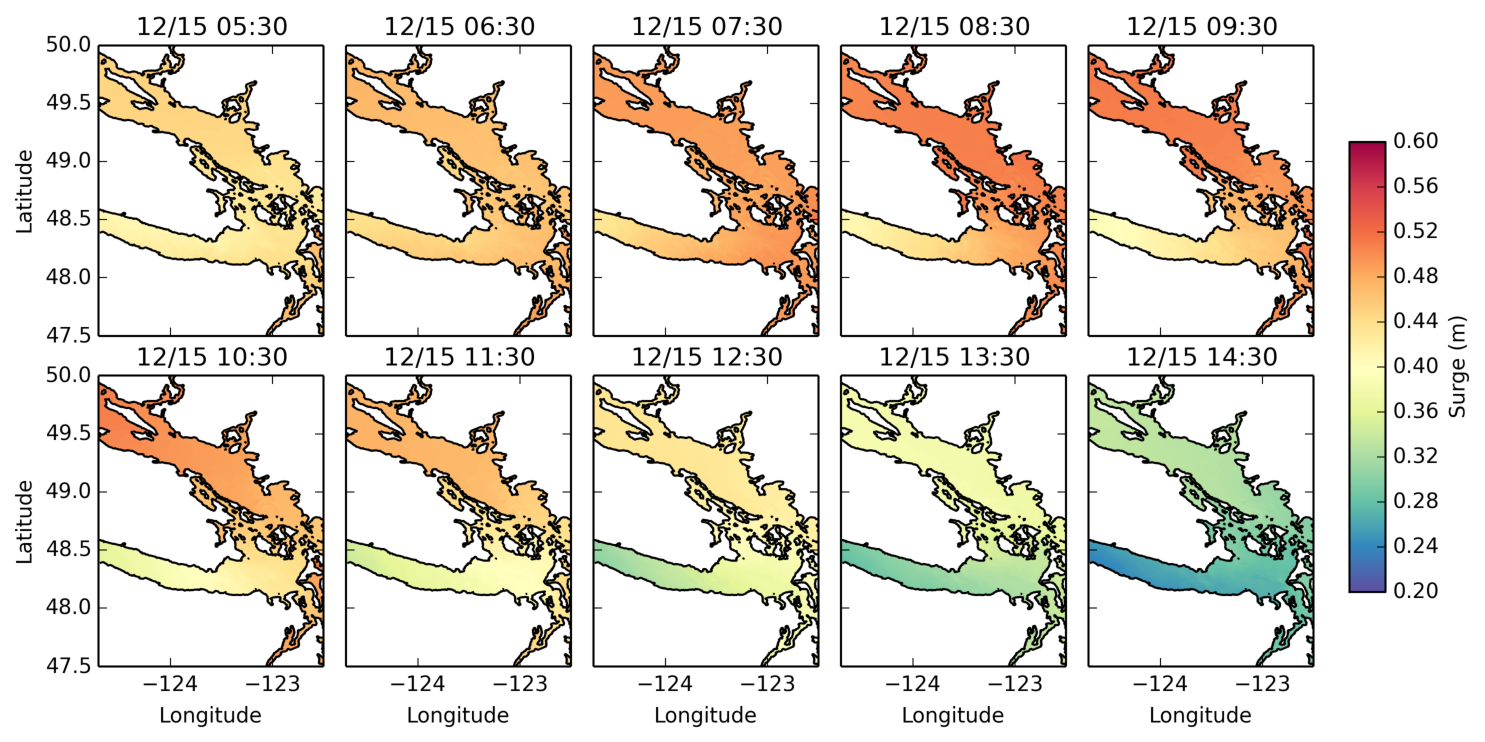
\includegraphics[scale=0.6]{Figures/dec2006_spatial_sshonly.pdf}
\caption{As in Figure \ref{fig:spatial} but for a simulation that does not include atmospheric forcing. }
\label{fig:spatial_sshonly}
\end{figure}

\subsection{Strong Wind Event}\label{sec:wind}
Next, a relatively strong wind event recorded at Point Atkinson on Nov 19, 2009 is considered. Although large wind speeds were observed, the surge associated with this event is rather small when compared to the previous cases (Figure \ref{fig:nov2009}). Two significant surge events are noted, the first occurring on Nov 19 with an observed amplitude of about 50 cm at Point Atkinson, and a second, larger surge of 62.5 cm on Nov 20. Surprisingly, the strong wind event of Nov 19 was associated with the smaller of the two surges. Neither of the surges occurred during a high tide and so no high water level events were recorded. Although not shown here, the other three locations also observed a maximum surge on Nov 20, which appears to be linked to a secondary high wind event and another surge entering the system at Tofino and Port Hardy. 

\citet{danard2003storm} discuss the role of wind fetch, the distance over which wind acts on the surface of a water basin, in setting up seiche motion in lakes and its contribution to storm surges. As wind blows over the surface of a lake, the water level becomes elevated on the downwind side and depressed on the upwind side in response to the wind-induced currents. The longer the fetch, the more significant the tilting of the water surface. These changes in water level can also contribute to storm surges.  During the high wind events on Nov 19 and Nov 20, the winds at Point Atkinson were directed to the west, explaining the lack of strong surge observed during this event since wind stresses would act to depress the water on the east side of the basin. In fact, the surge amplitude at Victoria on Nov 20 was 64.7 cm which is slightly higher than that observed at Point Atkinson (62.5 cm). Of the cases considered so far, this is the only example where the surge amplitude at Victoria was higher than that at Point Atkinson. The model results do not reflect a higher surge at Victoria (46.1 cm versus 50.5~cm at Point Atkinson), perhaps due to an underestimate in the wind speed and some discrepancies in the wind direction of the atmospheric forcing.  


\begin{figure}
\centering
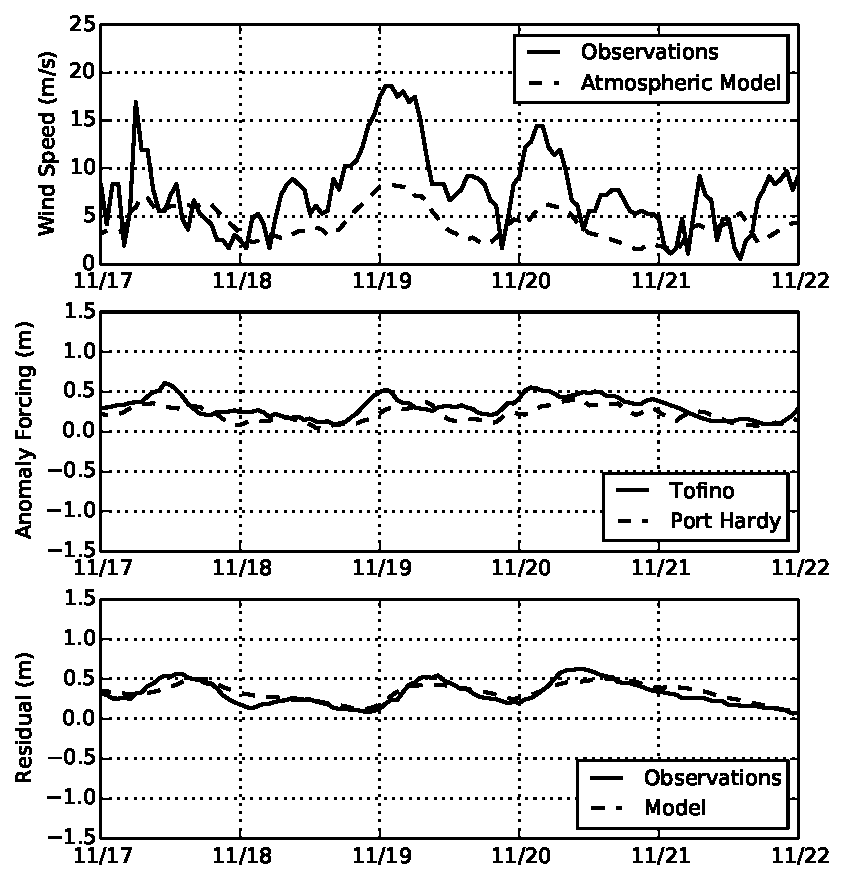
\includegraphics[scale=0.6]{Figures/nov2009.pdf}
\caption{Wind and storm surge conditions at Point Atkinson for a strong wind event on Nov 19, 2009. Top: Wind speed from Environment Canada observations \citep{ECClimateArchive} at Point Atkinson (solid) and from the atmospheric model (CGRF) at a grid point near Point Atkinson (dashed). Middle: Sea surface height anomaly at Tofino (solid) and Port Hardy (dashed) used as forcing conditions at the western and northern open boundaries. Bottom: Observed (solid) and modelled (dashed) residuals at Point Atkinson.  }
\label{fig:nov2009}
\end{figure}

The modelled water levels and residuals are too high for this hindcast, except at Victoria (Table \ref{tab:statistics}). Although Victoria has the smallest mean error in both the water level and residuals, its Willmott skill score and $\gamma^2$ values rank low when compared to the other stations. Generally, the skills scores are very good, scoring above 0.91 at all stations. 


\subsection{High Resolution Atmospheric Forcing}\label{sec:res}
The above comparison between the modelled and observed winds at Point Atkinson suggests that the atmospheric forcing product (CGRF) may not be adequate to produce accurate storm surge hindcasts since the wind speeds are substantially lower than observed. CGRF is a global atmospheric reforecasting model with horizontal resolution approximately 33 km over the Salish Sea domain, which is problematic since the Strait of Georgia itself is only about 30 km wide. As such, there are only one or two grid cells that are entirely over water in our domain, resulting in overly damped wind speeds at grid points close to land such as Point Atkinson. To determine the effect of under-resolved wind forcing on the storm surge hindcasts we compare simulations that have been forced with 1) the low resolution CGRF model and 2) a high resolution (2.5 km) HRDPS model from Environment Canada.  These simulations are performed for a storm surge that occurred on Dec 17, 2012 and cover the time period Dec 14-19, 2012. The high resolution product is not available for the hindcasts already discussed. 

First, a comparison of the wind speed and direction for the two models and observations is provided in Figure \ref{fig:dec2012_weather} at Point Atkinson and at Sandheads, a lighthouse station in the southern Strait of Georgia. For each of the models, the wind speed and direction at the closest grid point to the longitude/latitude of Point Atkinson and Sandheads is used for comparison. Although the low resolution CGRF model has a grid spacing of 33 km, two grid points align closely with these locations. At Point Atkinson, the high resolution model is in very good agreement with observations for both the wind speed and direction, however, the low resolution CGRF model significantly underestimates the wind speed during high wind periods on Dec 15, 2012 and Dec 17, 2012. At Sandheads, both the low resolution and high resolution models have good agreement with observations. The low resolution model has a very good match at Sandheads likely because this grid cell happens to be mostly over water. Although not shown here, both models have a similar sea level atmospheric pressure at these two locations. Note that data assimilation is used in the parent model of the nested HRDPS product.

\begin{figure}
\centering
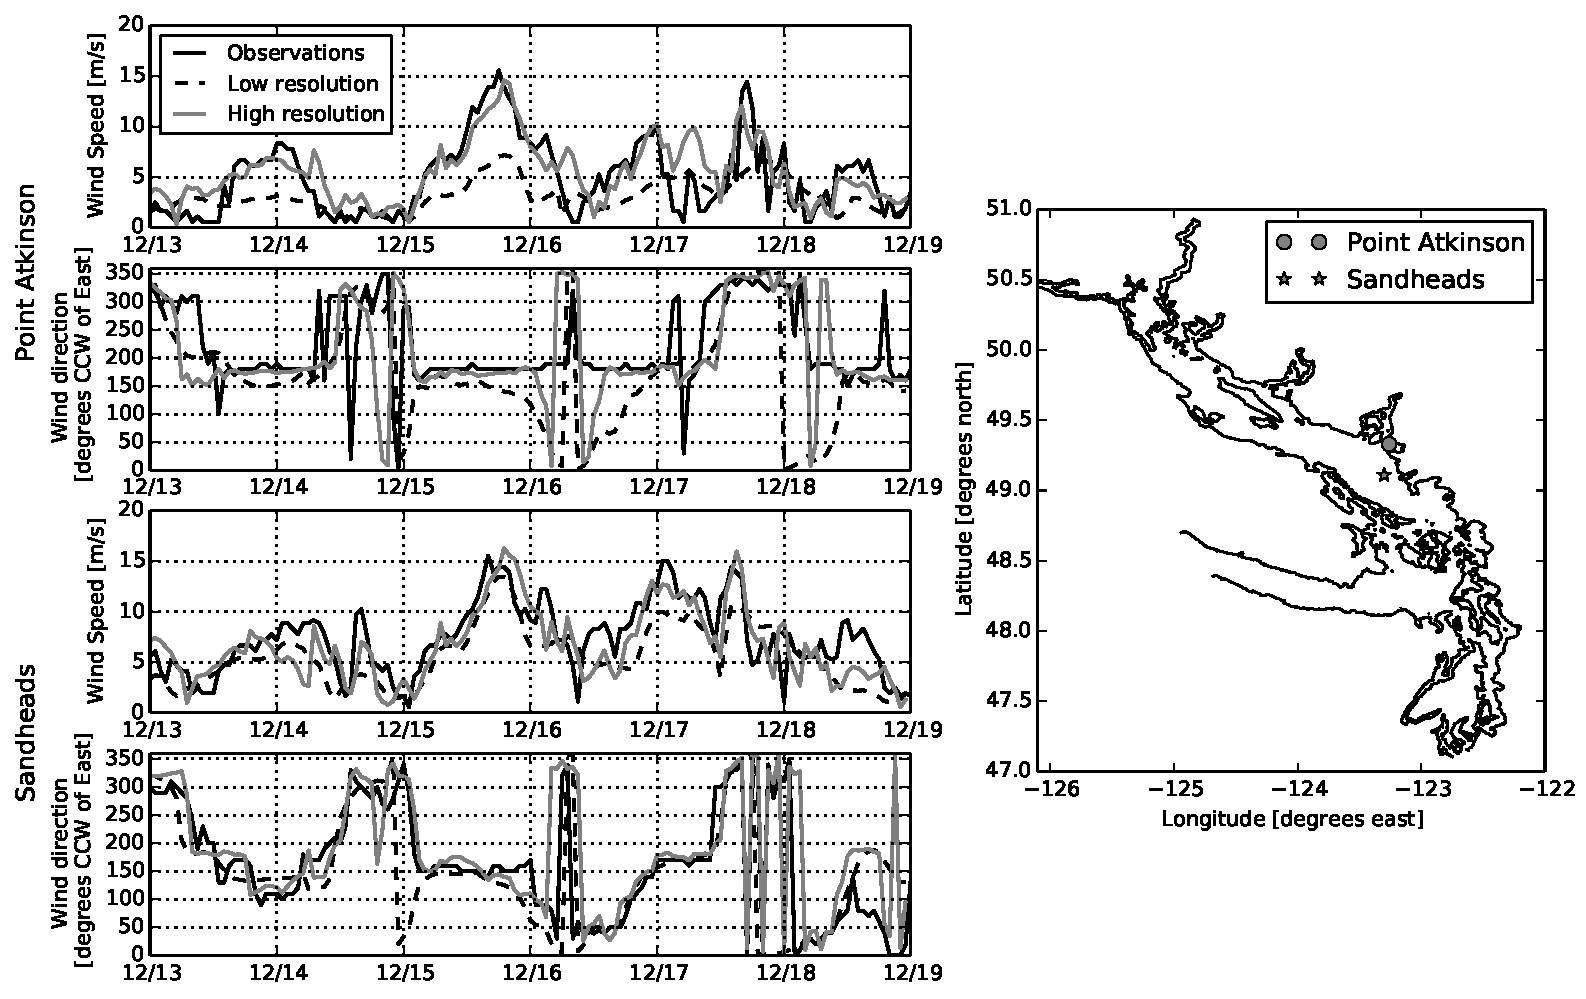
\includegraphics[scale=0.6]{Figures/dec2012_weather.pdf}
\caption{{\color{red}Comparison of observed and modelled winds during Dec 2012 storm surge simulation at Point Atkinson (top), Sandheads (middle) and NOAA Buoy 46087 (bottom). Observed winds shown in solid black, low resolution CGRF model in dashed black and high resolution model in grey. Observations from Sandheads and Point Atkinson are from the Environment Canada Climate Data archives \citep{ECClimateArchive}.  Observations at the NOAA Buoy are found at this url: \url{http://www.ndbc.noaa.gov/station_page.php?station=46087}. Wind direction represents the direction that the wind is headed.} }
\label{fig:dec2012_weather}
\end{figure}

Hindcasts with both atmospheric forcing products agree well with the observations (Figure \ref{fig:dec2012_surge}). Willmott skill scores for both modelled residuals are above 0.92 at these four locations. Further, the modelled residuals deviate only slightly from each other, most noticeable at Point Atkinson during the large wind event on Dec 15, 2012 where simulation with the low resolution atmospheric forcing has a residual that is 5 cm higher. Although the wind speeds on Dec 15, 2012 are quite high, this event did not result in any flooding or residuals greater than 50 cm. Significant flooding occurred later, on Dec 17, 2012, where the observed surge amplitude at Point Atkinson was 68.3 cm. Even though the low resolution model significantly under predicts the wind speed at some locations, it performs comparably to forcing with high resolution products. Much of the fine scale detail offered by the high resolution atmospheric model is averaged out since, to first order, the storm surge is a spatial integral of the wind. This result further demonstrates that the local wind is not the most important factor for setting up storm surges over this domain; however, local wind patterns contribute to wave conditions which can impact flooding and are not accounted for in this model. 

\begin{figure}
\centering
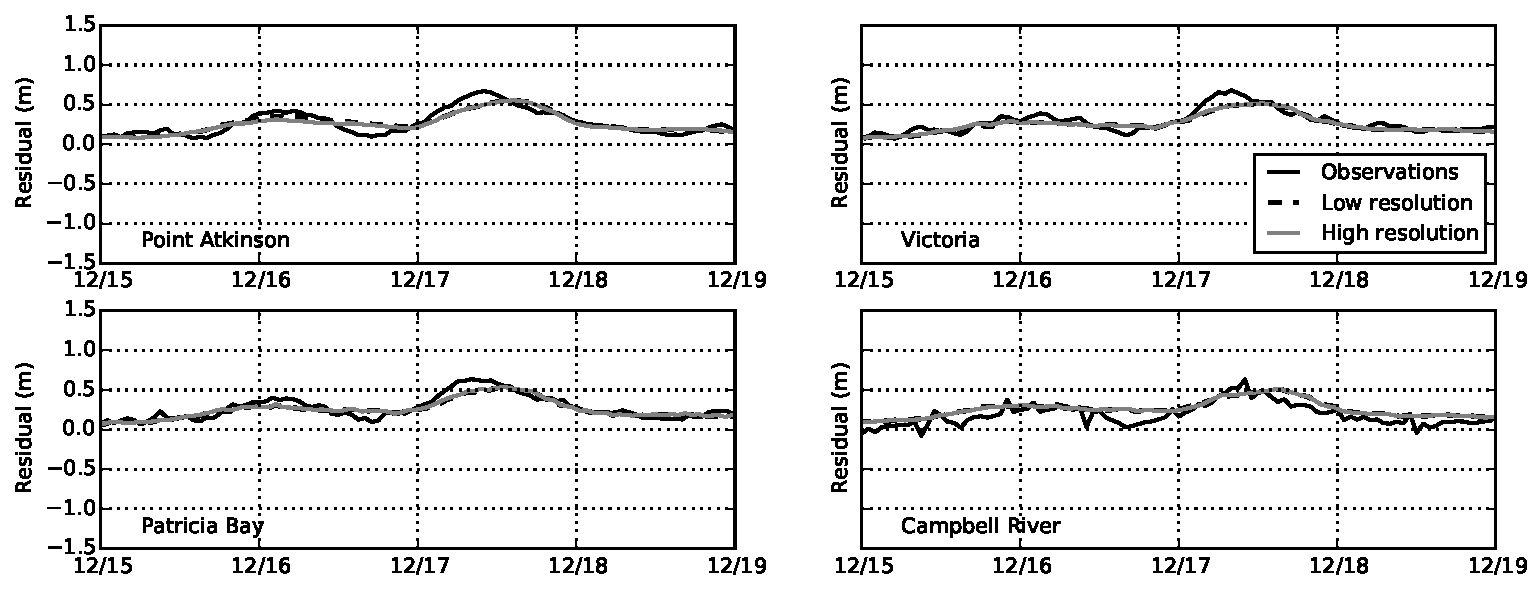
\includegraphics[scale=0.6]{Figures/dec2012_surge.pdf}
\caption{Comparison of observed (solid black) and modelled residuals for the Dec 2012 storm surge simulation. Modelled residuals from two simulations using a low resolution (dashed) and high resolution (grey) atmospheric products are shown. }
\label{fig:dec2012_surge}
\end{figure}

\section{Conclusion and discussion}\label{sec:diss}
In this article, we describe a three-dimensional numerical ocean model of the Salish Sea for accurate hindcasts of storm surges in the Strait of Georgia. The model is forced with eight tidal constituents at the western and northern open boundaries, as well as sea surface height anomaly from de-tided observations at Tofino and Port Hardy. Additionally, wind stress and local atmospheric pressure forcing were used at the ocean surface using an atmospheric reforecasting product called CGRF \citep{smith2014new}. Storm surge simulations began with zero initial conditions for the currents and sea surface height and were commenced several days prior to the event of interest to spin up the velocity fields. 

Hindcasts of five significant events in February 2006, November 2006, December 2006, November 2009, and December 2012 were simulated. In general, the model performs well at reproducing the observed water level heights and residuals, with Willmott skill scores greater than 0.88 in all cases and generally higher skill scores for the water level heights.  Further, in a single simulation, the skill scores are fairly consistent between the four stations examined. We have also assessed the relative importance of different forcing factors contributing to the storm surge. The sea surface height anomaly entering the system from the Pacific Ocean, or remote forcing,  contributes most significantly to the surge amplitude, in agreement with previous studies in this region \citep{murty1995storm}. Although the large scale wind patterns and atmospheric conditions are important in setting up the surge on the Pacific Ocean boundaries, the local winds within the Strait of Georgia are not the leading order contribution to surge amplitude. However, the local wind patterns can set up small spatial differences in the surge, resulting in higher surges on the mainland side of the Strait of Georgia due to the usually southerly winds during storm surge season. {\color{red}Additionally, surge amplitudes in the Strait of Georgia are typically higher than those in the Strait of Juan de Fuca, perhaps due a partial reflection of the surge from the mainland coast.} Results from an additional simulation with no tidal forcing but only surge propagation and atmospheric forcing found that nonlinear effects due to the tide-surge interaction were most important north of the San Juan and Gulf Islands. The modelled surge amplitude increased by about 10\% at Point Atkinson when the tide-surge interaction was neglected in one example. 

Comparisons between high resolution and low resolution atmospheric forcing further suggest that local winds are not the leading order factor in setting up large surge amplitudes. The low resolution model significantly underestimated wind speeds in certain areas of the domain, however, it performed just as accurately in reproducing surge amplitudes as the high resolution product.  Although the high resolution model delivers fine scale detail and more accurate local wind patterns, it did not provide any improvement to the surge hindcast. Since both of these products provide the same level of accuracy for storm surge hindcasts, in the future we will use the high resolution atmospheric model to produce real-time storm surge predictions, even though most of our testing was performed with the low resolution model. Additionally, the sea surface height anomaly from Neah Bay, forecasted by the National Oceanic and Atmospheric Administration (NOAA), will be used in future real-time water level predictions during the storm surge season. 

Several factors considered in other storm surge modelling studies have been neglected in these simulations. Primarily, effects due to wetting and drying have not been included. This is an important factor to consider in shallow, low lying areas where water levels retreat significantly to reveal land. In this article, the four locations used to assess storm surge accuracy are not in shallow regions and so wetting and drying is not considered to be important. However, several communities in the Strait of Georgia, such as Boundary Bay and Crescent Beach, are in shallow regions and are typically most affected by storm surge during the winter season. As such, efforts to include wetting and drying will be considered in the future. Additionally, flooding effects due to wave run up is left for a more detailed inundation study with higher resolution in the near-shore areas. Local winds have a significant impact on wave action which is a primary concern for flooding management. Further, the remote forcing is applied uniformly across the open boundary and so any spatial variability in the incoming surge are not accounted for in the model. Since the remote forcing is an important contributing factor, any forecasting with this regional model must make use of results from a larger scale prediction system.  

Since the Strait of Georgia is a large, semi-enclosed body of water storm surges can behave and evolve differently than in other coastal regions. For instance, the complicated coastlines and local wind patterns result in important spatial variations in the surge amplitude. As such, the strong wind caused by a large storm is not the only factor to be considered in community preparedness for surge conditions. The geometry of the Strait and local wind patterns render communities on the mainland side of the southern Strait of Georgia more susceptible to surges. Additionally, communities such as Campbell River are at risk due to the long fetch and predominately southerly winds during the winter months.

Finally, difficulties in reproducing accurate M$_2$ tidal harmonics in both the Strait of Georgia and the Strait of Juan de Fuca have been highlighted in this study among others \citep{stronach1993update, foreman2004m}. Future work will attempt to improve model accuracy by examining mixing parametrizations and energy dissipation due to bottom friction and their effect on tidal harmonics. Additionally, a biological-chemical modelling component will be added. 


%future directions: running real time, biology and chemistry, model improvements?
%summary of skill scores



\appendices
\section{Details on tidal tuning}\label{sec:appendix}
This section details the procedure used to tune the tidal forcing for a good match with observations in the Strait of Georgia. Originally, the eight most important tidal constituents were extracted from a tide prediction tool called Webtide \citep{webtide} at the western Juan de Fuca boundary based on work by \citet{foreman2000webtide}. At the northern boundary,  M$_2$ and K$_1$ tidal harmonics for both elevation and currents were taken from \citet{thomson1980johnstone}, as well as elevation harmonics for O$_1$ and S$_2$. The remaining constituents were extrapolated from Webtide based on the ratio between S$_2$/M$_2$ amplitudes and phase differences for the semi-diurnal constituents and O$_1$/K$_1$ for the diurnal constituents. However, these forcing conditions did not result in a good match between observed and modelled tidal elevation harmonics in the Strait of Georgia, the main region of interest (although the matches in the Strait of Juan de Fuca were adequate). As such, tidal forcing was tuned, by first adjusting the western boundary M$_2$ and K$_1$ phase and K$_1$ amplitude for a good match in the Strait of Georgia (specifically at Point Atkinson, Gibsons Landing, Winchelsea and Halfmoon Bay). This tuning was performed on simulations that used only M$_2$ and K$_1$ forcing. Next, the M$_2$ and K$_1$ fluxes at the northern boundary were adjusted because the cross-sectional area of transect used by \citet{thomson1980johnstone} to measure tidal currents in Johnstone Strait is smaller than the cross-sectional area of our northern boundary. Finally, the remaining constituents were added, starting with O$_1$, then S$_2$, and then in pairs P$_1$/N$_2$ and Q$_1$/K$_2$. Final adjustments were made by slightly varying amplitude and phase, evaluating the changes to M$_2$, K$_1$ and the ratios S$_2$/M$_2$, N$_2$/M$_2$, K$_2$/M$_2$, O$_1$/K$_1$, P$_1$/K$_1$, Q$_1$/K$_1$ and then choosing new values to move closer to observations by linear interpolation. 

Below, Table \ref{tab:comparison} compares the M$_2$ and K$_1$ elevation harmonics with data from \citet{foreman1995tidal}, \citet{foreman2004m} and \citet{foreman2012circulation}. Overall, the average complex difference for M$_2$ is 8.05 cm and for K$_1$ is 2.58 cm, but both constituents perform very well in the Strait of Georgia region. 

\begin{table}[h]
\centering 
\tbl{Comparisons of modelled and observed amplitudes and phases. $R$ is the ratio of modelled to observed amplitude. $\Delta \phi$ is the difference between modelled and observed phase. $D$ is amplitude of the complex difference. The mean error and root mean square (RMS) error are calculated as the difference between the modelled quantity and observed quantity. }
{\begin{tabular}{l l l l c c c c c c} 
\hline 
& & & & \multicolumn{3}{c}{M$_2$} & \multicolumn{3}{c}{K$_1$} \\ 
\hline 
            & Station name     & Longitude & Latitude & $R$ & $ \Delta \phi$ (deg) & $D$ (cm) & $R$ & $ \Delta \phi$ (deg) & $D$ (cm) \\
\hline 
1 & Port Renfrew & -124.43 & 48.55 & 1.16 & -9.4 & 16.63  & 1.03 & -4.94 & 4.17 \\
2 & Sheringham Point & -123.92 & 48.38 & 1.19 & -16.47 & 17.95  & 1 & -4.44 & 4.24 \\
3 & Pedder Bay & -123.55 & 48.33 & 0.96 & -27.39 & 15.91  & 0.99 & -2.41 & 2.66 \\
4 & Esquimalt & -123.43 & 48.43 & 0.91 & -23.09 & 14.40  & 0.99 & -1.04 & 1.21 \\
5 & Victoria & -123.37 & 48.42 & 0.89 & -17.77 & 11.62  & 1.04 & -1.83 & 3.22 \\
6 & Clover Point & -123.35 & 48.41 & 0.83 & -17.95 & 13.39  & 1.03 & -2.23 & 3.14 \\
7 & Finnerty Cove & -123.3 & 48.47 & 0.83 & -8.24 & 9.47  & 1.02 & -2.19 & 3.25 \\
8 & Fulford Harbour & -123.45 & 48.77 & 0.82 & -3.08 & 10.78  & 1 & -0.63 & 0.83 \\
9 & Tumbo Channel & -123.11 & 48.79 & 1.05 & 2.03 & 4.43  & 1.04 & 0.66 & 3.34 \\
10 & Patos Island & -122.97 & 48.78 & 1.03 & 0.26 & 2.32  & 1.04 & -1.5 & 3.92 \\
11 & Whaler Bay & -123.33 & 48.89 & 1 & -0.76 & 1.10  & 1.01 & -0.48 & 1.19 \\
12 & Tsawwassen & -123.13 & 48.99 & 1 & 0.92 & 1.31  & 1.01 & 0.19 & 1.09 \\
13 & Sandheads & -123.3 & 49.1 & 1.02 & -1.05 & 2.58  & 1.04 & -0.59 & 3.15 \\
14 & Point Grey & -123.27 & 49.25 & 0.98 & -3.31 & 5.83  & 0.96 & -0.68 & 3.63 \\
15 & Point Atkinson & -123.25 & 49.33 & 1.01 & -0.48 & 1.07  & 1 & -0.56 & 0.94 \\
16 & Gibsons Landing & -123.5 & 49.4 & 0.98 & 0.75 & 2.34  & 1 & 0.96 & 1.47 \\
17 & Winchelsea & -124.08 & 49.3 & 1.01 & -0.19 & 0.78  & 1.01 & 0.51 & 1.30 \\
18 & Halfmoon Bay & -123.92 & 49.52 & 1.01 & -0.15 & 0.83  & 1.01 & 0.15 & 0.72\\ 
19 & Irvines Landing & -124.05 & 49.63 & 1 & -0.32 & 0.59  & 1.01 & 0.24 & 1.12 \\
20 & Powell River & -124.55 & 49.86 & 1 & -1.72 & 3.05  & 1 & -0.01 & 0.43 \\
21 & Little River & -124.92 & 49.74 & 1.03 & 0.07 & 2.54  & 1.01 & 0.33 & 0.73\\ 
22 & Lund & -124.76 & 49.98 & 1.02 & -2.52 & 4.98  & 1.02 & -0.95 & 2.45 \\
23 & Twin Islets & -124.93 & 50.03 & 1.02 & -2.05 & 4.22  & 1.01 & -0.24 & 0.72\\ 
24 & Campbell River & -125.24 & 50.04 & 0.99 & 0.51 & 1.12  & 1 & 0.94 & 1.39 \\
25 & Maude Island E & -125.33 & 50.13 & 1.13 & -10.02 & 12.62  & 0.97 & -1.44 & 2.89\\ 
26 & Nymphe Cove & -125.36 & 50.13 & 1.02 & -5.43 & 6.04  & 0.97 & -0.29 & 2.02 \\
27 & Seymour Narrows & -125.34 & 50.13 & 0.63 & 31.31 & 53.40  & 1.14 & 10.91 & 17.28 \\
28 & Brown Bay & -125.37 & 50.16 & 0.98 & -5.63 & 9.26  & 0.98 & -0.04 & 1.17 \\
29 & Chatham Point & -125.44 & 50.33 & 1.09 & -5.49 & 12.18  & 0.98 & -3.18 & 3.85 \\
30 & Kelsey Bay & -125.96 & 50.39 & 1 & -1.69 & 3.50  & 0.98 & -0.39 & 1.00 \\
31 & Yorke Island & -125.97 & 50.44 & 0.99 & 1.59 & 3.32  & 1.01 & 1.23 & 1.37\\ 
\hline 
&   Mean Error (cm/deg) & & & 4.23  & 6.5 & 8.05   & 1.56 & 1.49 & 2.58 \\
&   RMS Error (cm/deg)  & & & 7.67  & 10.73 & 12.73 & 2.41 & 2.57 & 3.91 \\
\hline  
\end{tabular}}
\label{tab:comparison} 
\end{table}


\section*{Acknowledgements}\label{sec:ack}
We would like to thank Michael Foreman, Diane Masson, Luc Fillion, Rich Pawlowicz, Mark Halverson, Kao-Shen Chung, and Pramod Thupaki for providing data used in model set up and evaluation. For providing guidance with stakeholder engagement, we also thank Stephanie Chang, Jackie Yip, and Shona van Zijil de jong. This research was enabled in part by support provided by WestGrid (www.westgrid.ca) and Compute Canada Calcul Canada (www.computecanada.ca).

\section*{Funding}
This project is funded by the Marine Environmental Observation Prediction and Response Network (MEOPAR), a Network of Centres of Excellence of Canada.

\bibliographystyle{apacite}
\bibliography{ref}

\end{document}



